\documentclass[print]{elsarticle}
\usepackage{amsmath, amssymb}
\usepackage{breqn}
\usepackage{booktabs}
\usepackage{graphicx}
\usepackage[utf8]{inputenc}
\usepackage[T1]{fontenc}
\usepackage[pdftex]{color}
\usepackage[font=footnotesize, labelfont=bf]{caption}
\usepackage{geometry}
\usepackage{siunitx}
\usepackage{hyperref}
\usepackage{epstopdf}
\usepackage[labelfont=bf,textfont={sl,bf},lofdepth,lotdepth]{subfig}
\usepackage{cleveref}
%%%%%%%%%%%%%%%%%%%%%%%%%%%%%%%%%%%%%%%%%%%%%%%%%%%%%%%%%%%%%%%%%%%%%%%%%%%%%%%%%%%%%%%%%%
%                                  MODIFICACIONES                                        %
%%%%%%%%%%%%%%%%%%%%%%%%%%%%%%%%%%%%%%%%%%%%%%%%%%%%%%%%%%%%%%%%%%%%%%%%%%%%%%%%%%%%%%%%%%
\oddsidemargin=1cm
\textwidth=14cm
%%%%%%%%%%%%%%%%%%%%%%%%%%%%%%%%%%%%%%%%%%%%%%%%%%%%%%%%%%%%%%%%%%%%%%%%%%%%%%%%%%%%%%%%%%
%                                 FORMATOS                                               %
%%%%%%%%%%%%%%%%%%%%%%%%%%%%%%%%%%%%%%%%%%%%%%%%%%%%%%%%%%%%%%%%%%%%%%%%%%%%%%%%%%%%%%%%%%
\DeclareMathAlphabet{\mathpzc}{OT1}{pzc}{m}{it}
\newtheorem{dfn}{Definition}
\newtheorem{thm}{ THEOREM}[section]
\newtheorem{pro}{ PROPOSITION}[section]
\newtheorem{lem}{ LEMMA}[section]
\newtheorem{definition}{ DEFINITION}[section]
\newtheorem{corollary}{ COROLLARY}[section]
\newtheorem{consequence}{ CONSEQUENCE}[section]
\newtheorem{remark}{ REMARK}[section]
\newtheorem{example}{\bf Example}[section]
\newtheorem{proof}{\bf Proof}[section]
\newproof{pf}{Proof}

\newcommand{\fin}{\vrule height3pt width3pt depth2pt}
\newcommand{\normL}[1]{\left[\mathbb{E}\left|#1\right|^2\right]^{1/2}}
\newcommand{\ms}[1]{\mathbb{E}\left|#1\right|^2}
\newcommand{\mep}[1]{\mathbb{E}|#1|^p}
\newcommand{\m}[1]{\mathbb{E}#1}
\newcommand{\meanp}[2]{\mathbb{E}\left|#1\right|^{#2}}
\newcommand{\condexp}[2]{\mathbb{E}\left[#1|#2\right]}
\newcommand{\lftrght}[3]{\left#2 #1\right #3}\DeclareMathOperator{\tr}{tr}
\DeclareMathOperator{\diag}{diag}
%opening
%\title{Important Simulation Examples for the Stochastic Steklov Scheme}
%\author[sj]{S. D\'{\i}az-Infante}
%\ead{sauld@cimat.mx}
%\author[sj]{S. Jerez}
%\ead{jerez@cimat.mx}

\begin{document}
	\begin{frontmatter}
		\title{Convergence and Asymptotic Stability  of  the Explicit
		Steklov Method for Stochastic Differential Equations 
		\tnoteref{t1}
		}%,t2}}
		\tnotetext[t1]{This work has been partially
		supported by CONACYT project *****
		}
		\author[sj]{S. D\'{\i}az-Infante}
		\ead{sauld@cimat.mx}
		\author[sj]{S. Jerez}
		\ead{jerez@cimat.mx}
		%\context[cor1]{Corresponding author. Tel.: +52 473 732 7155; fax: +52 473 732 5749.}
		\address[sj]{
		Department of Applied Mathematics, CIMAT, Guanajuato, Gto., Mexico,
		36240.
		}
		\begin{abstract}
			In this document, we develop a set of examples where the Steklov Schemes can be applied
			with good results. The examples was taken from common and variated application areas.
		\end{abstract}
		\begin{keyword}
			stochastic differential equations, Steklov average,
			explicit methods, convergence, asymptotic stability,
		\end{keyword}
	\end{frontmatter}
	\section{Steklov Scheme Construction for SDE Systems }
		Consider the vector SDE
\begin{equation}\label{eqn:SDESystem}
	dy = f(y)dt + g(y)dW_t, \qquad y(0) = y_0,
\end{equation}
where $f:\mathbb{R}^d \to \mathbb{R}^d$, $g:\mathbb{R}^d \to \mathbb{R}^{d \times m}$, 
$W$ is a standard $m$-dimensional Brownian motion.
Assuming that $f =(f^{(1)},\dots f^{(d)})^T$ and $g = (g^{(1)}, \dots g^{(m)}) $ satisfy
the usual conditions for existence and uniqueness of solutions to \eqref{eqn:SDESystem}, 
we define for each $j =1,\dots, d$ the functional
$H^{(j)}: U\subset \mathbb{R}^d \to \mathbb{R}$ by
\begin{equation*}
	H^j(u) = \int \frac{du}{
		f^{(j)}(X^{(1)}_{0}, \dots, X^{(j-1)}_{0}, u, X^{{(j+1)}}_{0}, \dots,  X^{(d)}_{0})
	}.
\end{equation*}
Moreover, we assume that $H^{(j)}$ is integrable for all fixed $X_0 \in U$ and has inverse $[H^j]^{-1}$. 
So, we create a  Steklov scheme as follows.
For each component equation we solve the associated deterministic initial value problem
$$
	\frac{dx^{(j)}}{dt} = f^{(j)}(x), \qquad x^{(j)}(0)= x_0^j, \qquad j = 1, \dots, d
$$
with
\begin{align}\label{eqn:SteklovSchem1}
	\frac{x^{(j)}_{k+1} - x^{(j)}_{k} }{h}	&= \varphi_{f^{(j)}}(x^{(j)}_{k}, x^{(j)}_{k+1}) \notag \\
	\varphi_{f^{(j)}} \left(x^{(j)}_{k}, x^{(j)}_{k+1} \right) &= 
		\frac{x^{(j)}_{k+1} - x^{(j)}_{k} }{H(x^{(j)}_{k+1}) -H(x^{(j)}_{k})},	\\
		H^j(u) &= 
			\int 
				\frac{du}{
					f^{(j)}(x^{(1)}_{k+1}, \dots, x^{(j-1)}_{k+1}, u, x^{(j+1)}_{k}, \dots, x^{(d)}_{k})
				} \notag,
\end{align}
where, $x^{{(1)}}_{k+1}, \dots, x^{{(j-1)}}_{k+1}$ results from the first
$j-1$ schemes. In this way we get the explicit recurrence for each $j\in \{ 1,\dots d\}$
\begin{equation*}
	x_{k+1}^{(j)} = 
		[H^{(j)}]^{-1}
		\left(
			h + H^{(j)}\left(x_k^{(j)}\right)
		\right).
\end{equation*}
Finally we approximate the diffusion term of SDE \eqref{eqn:SDESystem} with a Euler-Maruyama scheme to produce
\begin{equation}\label{eqn:SteklovRecurrence}
	X_{k+1}^{(j)} = 
		[H^{(j)}]^{-1}
		\left(
			h + H^{(j)}
			\left(
				X_k^{(j)}
			\right)
		\right)
	+ g^{(j)} \left(X_k^{(j)} \right) \Delta W_k^{(j)}.
\end{equation}
However the necessary assumptions here would be so strong.
\subsection{Alternative Construction}
Here, we propose a way to weak the assumptions over the coefficients of SDE
\eqref{eqn:SDESystem}.
Suppose that for each $j \in \{1, \dots, d \}$ there are locally Lipschitz functions 
$a_1^{(j)}:\mathbb{R}^{d} \to \mathbb{R}$, \quad 
$a_2^{(j)}:\mathbb{R}^{d-1} \to \mathbb{R}$ such that 
\begin{equation}\label{eqn:AlternativeConstruction}
	f^{(j)}(y) = a_1^{(j)}(y)y^{(j)} + a_2^{(j)}(y^{(-j)}), \qquad
	y^{(-j)} = (y^{(1)}, \dots ,y^{(j-1)}, y^{(j+1)}, \dots, y^{(d)}).
\end{equation}
	Under this assumptions for each component equation take
\begin{align*}
	H^{(j)}(u)	&= \int \frac{du}{a_1^{(j)} u + a_2^{(j)}} 
		= \ln \left( a_1^{(j)} u + a_2^{(j)} \right),\\
	\left[H^{(j)}\right]^{(-1)} (v) & = \frac{\exp(a_1 v ) - a_2}{a_1}\\
	a_1^{(j)} &=
		a_1^{(j)}
			\left(
				x^{(1)}_{k+1}, \dots, x^{(j-1)}_{k+1},
				x^{(j)}_{k} , x^{(j+1)}_{k},\dots,x^{(d)}_{k}
			\right),
			\\
	a_2^{(j)} &=
		a_2^{(j)}
			\left(
				x^{(1)}_{k+1}, \dots, x^{(j-1)}_{k+1},
				x^{(j+1)}_{k},\dots,x^{(d)}_{k}
			\right).
	\end{align*}
Therefore, approximating the diffusion term in a similar way as as in the scheme \eqref{eqn:SteklovRecurrence} 
we define the Split Step Linear Steklov method (\SM) by
\begin{align}\label{eqn:SteklovSchem2}
	X^{(j)}_{k+1} %&= \left[ H^{(j)}\right ]^{(-1)} ( H^{(j)}(X_k) + h ) \notag	\\
			&=
			\left(
				X_k^{(j)} + 
				\frac{a_2^{(j)} }{a_1^{(j)}}
			\right) 
			\exp\left(
					a_1^{(j)}h
				\right) - \frac{a_2^{(j)}}{a_1^{(j)}} 
		+ g^{(j)}(X_k) \Delta W^{(j)}_k, \notag\\
	a_1^{(j)} &=
		a_1^{(j)}
			\left(
				X^{(1)}_{k+1}, \dots, X^{(j-1)}_{k+1},
				X^{(j)}_{k} , X^{(j+1)}_{k},\dots,X^{(d)}_{k}
			\right),
			\\
	a_2^{(j)} &=
		a_2^{(j)}
			\left(
				X^{(1)}_{k+1}, \dots, X^{(j-1)}_{k+1},
				X^{(j+1)}_{k},\dots, X^{(d)}_{k}
			\right). \notag
\end{align}
The rest of this document consist of a important set of examples.

			The Lotka-Volterra model 
\begin{align} %\label{eqn:DeterministicLotkaVolterra}
	\frac{dx}{dt} &= ax - bxy, \label{eqn:DetLotkaVolterraArnoldA}
	\\
	\frac{dy}{dt} &=-by +dxy,\label{eqn:DetLotkaVolterraArnoldB}
\end{align}
describes in a very simple way, the interaction of two populations. Usually, $x$, $y$, represent
the predator and prey populations, respectively. The linear terms $ax$, $-by$, describes the behavior
of a specie in the absence of the other, and the quadratic terms describes the interaction. 
Although this model has been criticized for being unrealistic, its simplicity permits
understand essential features of the predator-prey interaction \cite{may2001stability}. 

	For positive initial conditions,
all solutions, except the fixed-point $(\bar{x}, \bar{y})=(b/d, a/b)$, are periodic. However, the standard
procedures to form finite-difference schemes generally give numerical solutions that spiral into or away from the 
fixed-point. Mickens' \cite{Mickens2003} and Serghini's \cite{SerghiniMounim2004} methods, produce solutions that are 
periodic, being the 
second more precise. So, we compare the performance of the deterministic \SM method with 
these non-standard schemes see \Cref{fig:DeterministicLotkaVolterra}.
%\Cref{fig:DetPhasePotraitLotkaVolterraArnold},
%\Cref{subfig:DetX1LotkaVolterraArnold},
%\Cref{subfig:DetX2LotkaVolterraArnold}.

	However, in any real ecosystem are two sources of fluctuation \cite{may2001stability}:
\begin{inparaenum}[(i)]
	\item
		The population are finite and discrete, that is, its size change in integral steps. This
		is called demographic stochasticity or internal fluctuations.
	\item
		A realistic biological environment is not deterministic. Consequently, a better description
		should consider fluctuation in the phenomenological parameters like, growth rates, carrying capacities, etc.
		This kind of fluctuations is called external.
\end{inparaenum}

	Since the contribution of internal fluctuations decrease with the size of the population, usually, stochastic
models add randomness in the environmental parameters, see for example 
\cite{Bahar2004, Mao2002, Mao2003, Mao2009, Takeuchi2006, Rudnicki2007, Liu2013d, Yagi2011}. 
We consider the stochastic Lotka-Volterra model studied in \citet{Arnold1979}. 
Here, the authors suppose that the environmental fluctuations will mainly manifest in the growth rate $a$ with
$a\to a+\sigma dW_t$, where $a$ represents the mean grow rate and $\sigma^2$ controls the intensity of the 
white noise $dB(t)$. So, they obtain the following SDE:
\begin{align}
	dX^{(1)}_t &= X^{(1)}_t(a -b X^{(2)}_t) dt +\sigma X^{(1)}_t dW_t
	\label{eqn:StoLotkaVolterraArnold1} \\
	dX^{(2)}_t &= X^{(2)}_t( X^{(1)}_t - d).
	\label{eqn:StoLotkaVolterraArnold2}
\end{align}
With this on mind, taking
\begin{align*}
	a_1(x_k, y_k) &:= a - b y_k, & b_1(y_k):= 0,\\
	a_2(x_{k+1}, y_k) &:= b x_{k+1} -d, & b_2(y_k):= 0,
\end{align*}
in \eqref{eqn:SteklovSchem2}, we get the \SM method
\begin{align}
	X^{(1)}_{k+1} &= \exp \left[ a_1 \left( X^{(1)}_k,X^{(2)}_k \right) h \right] X^{(1)}_k 
		+\sigma X^{(1)}_k \Delta 	W_k,  \notag \\
%
	X^{(2)}_{k+1} &= \exp \left[ a_2\left(X^{(1)}_{k+1},X^{(2)}_k\right) h \right] X^{(2)}_k, \\
		a_1\left( X^{(1)}_k, X^{(2)}_k \right) &:= a - b X^{(2)}_k, \qquad
		a_2\left( X^{(1)}_{k+1}, X^{(2)}_k \right):= b X^{(1)}_{k+1} -d. \notag
\end{align}
In 
	\Cref{subfig:StoPhasePotraitLotkaVolterraArnold},
	\Cref{subfig:StoX1LotkaVolterraArnold}, and
	\Cref{subfig:StoX2LotkaVolterraArnold}
we compare the noisy trajectories produced with this scheme and the EM.

\begin{figure}[tb]
	\centering
	\subfloat[]{
		
		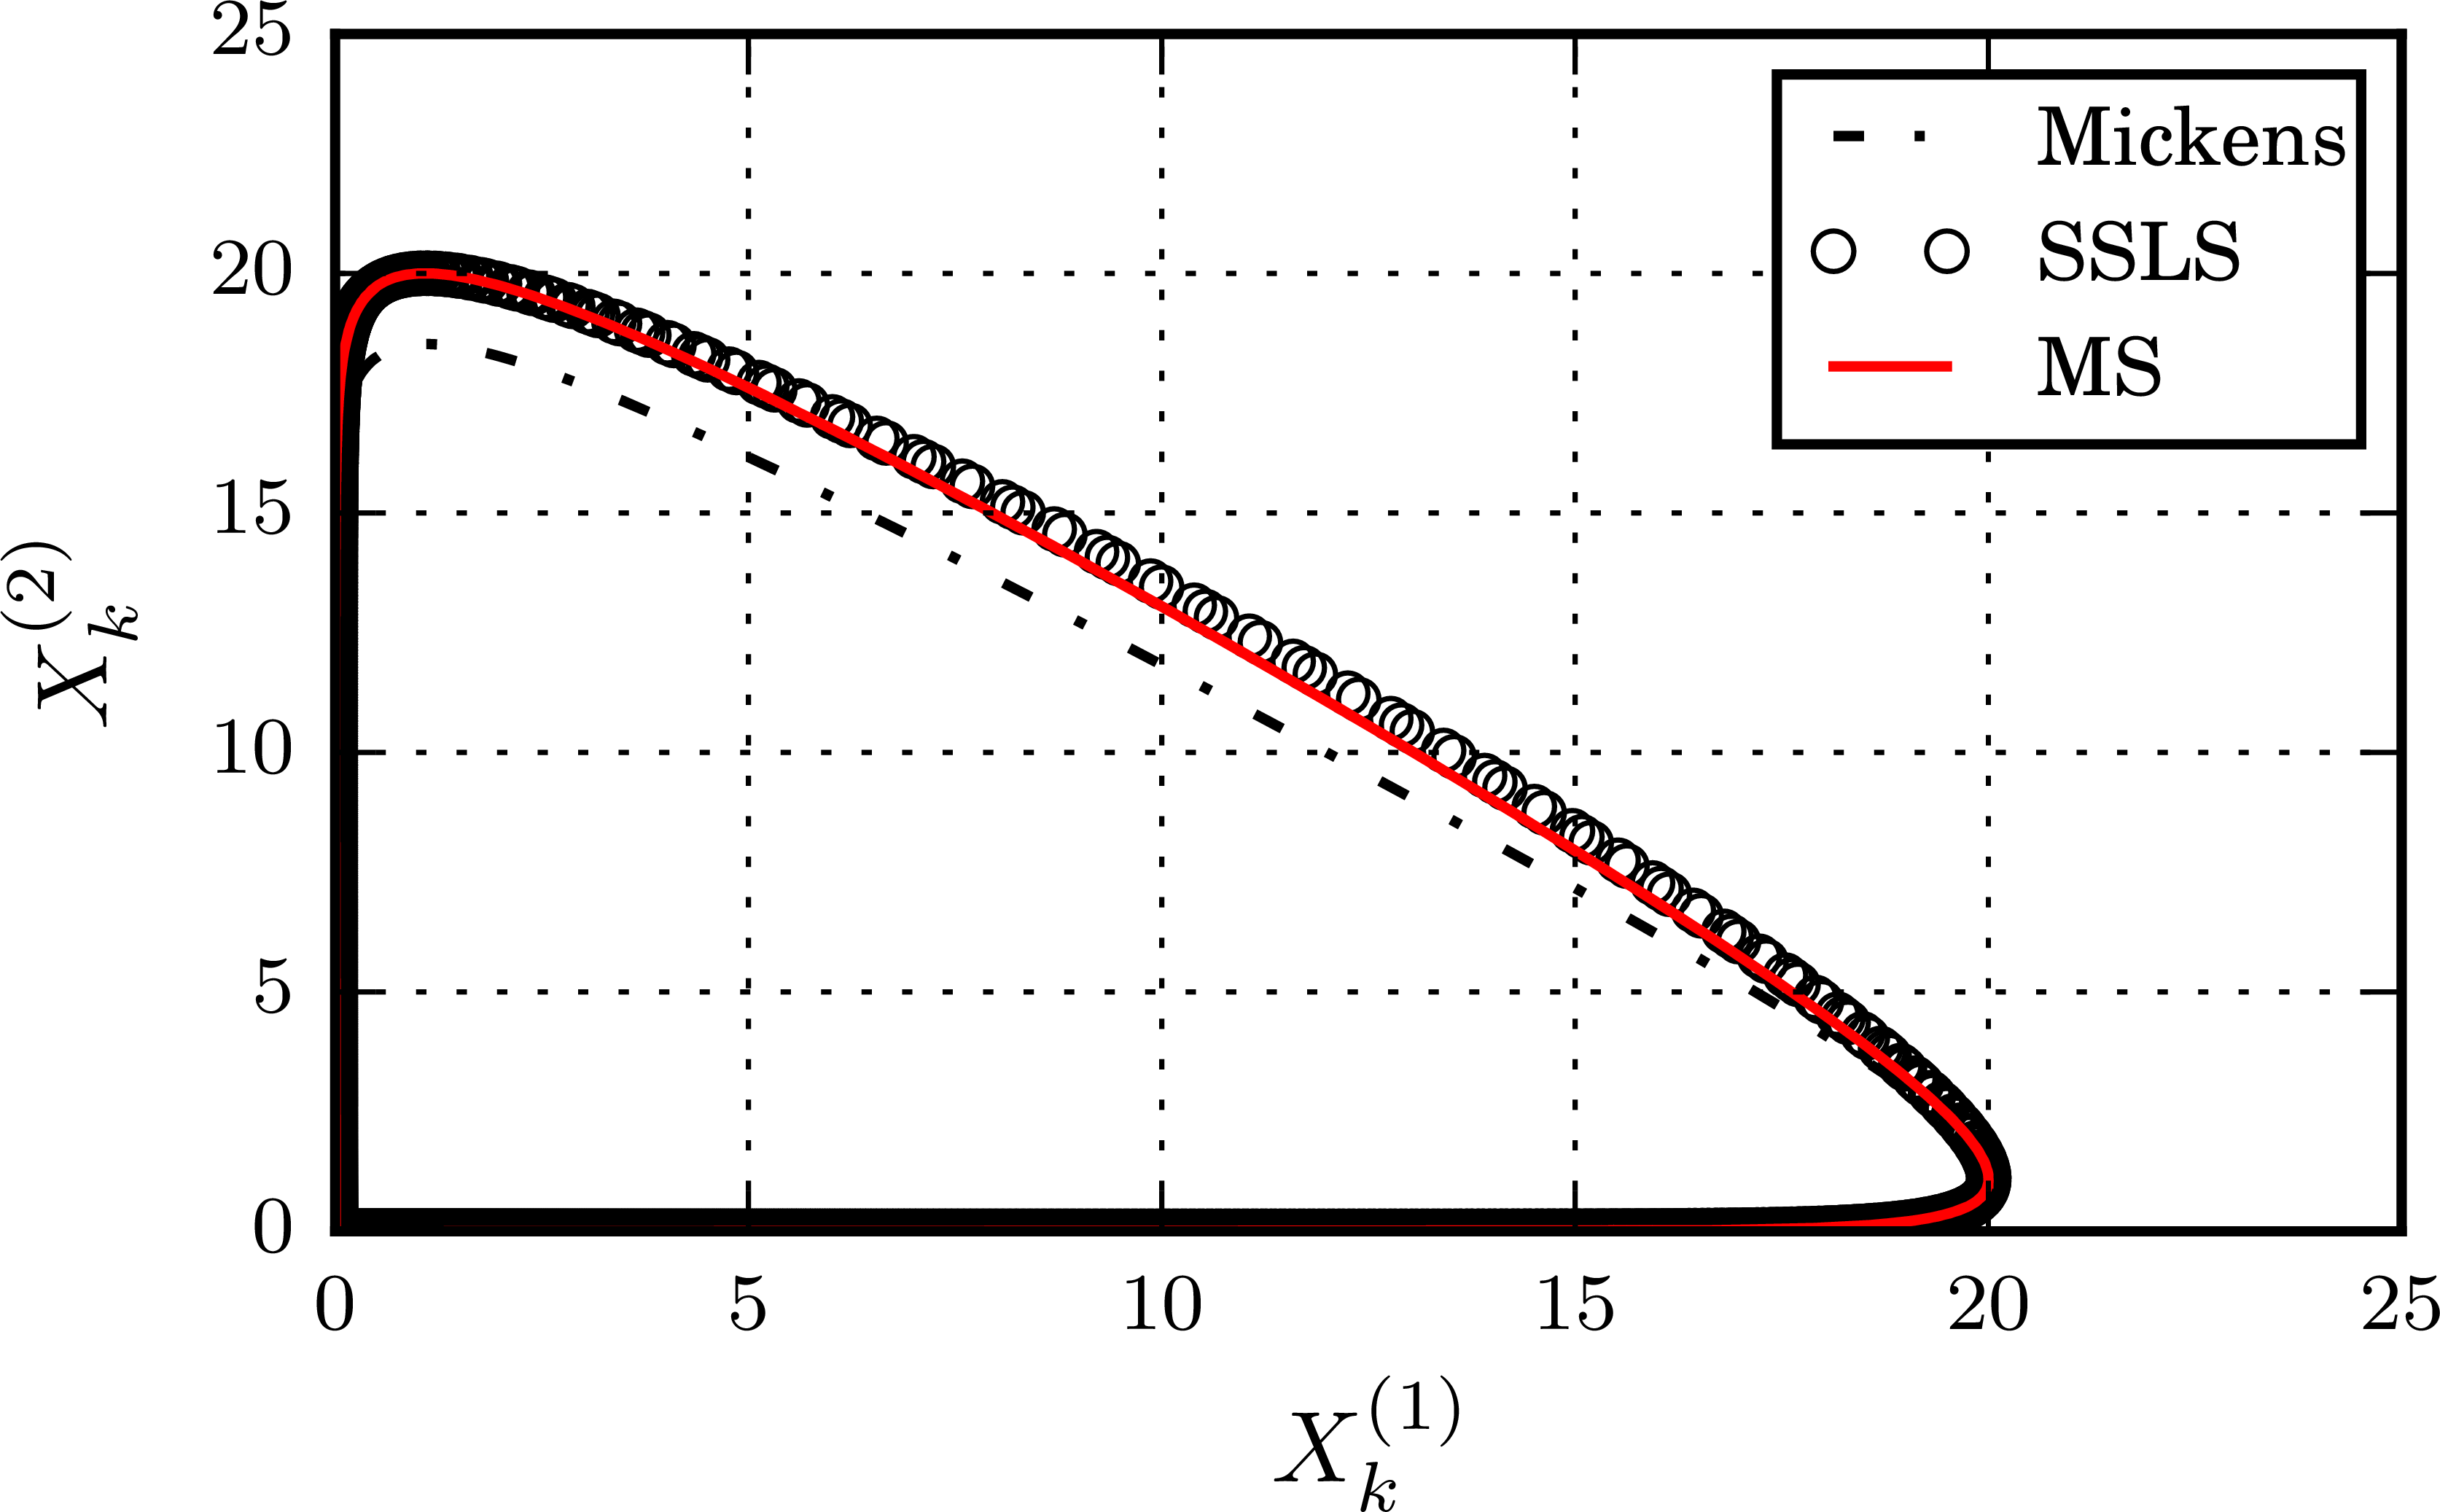
\includegraphics{./papers/paperB/figures/DetPhasePotraitLotkaVolterraArnold.png}
		\label{fig:DetPhasePotraitLotkaVolterraArnold}
	} \\
	\subfloat[]{
		\centering
		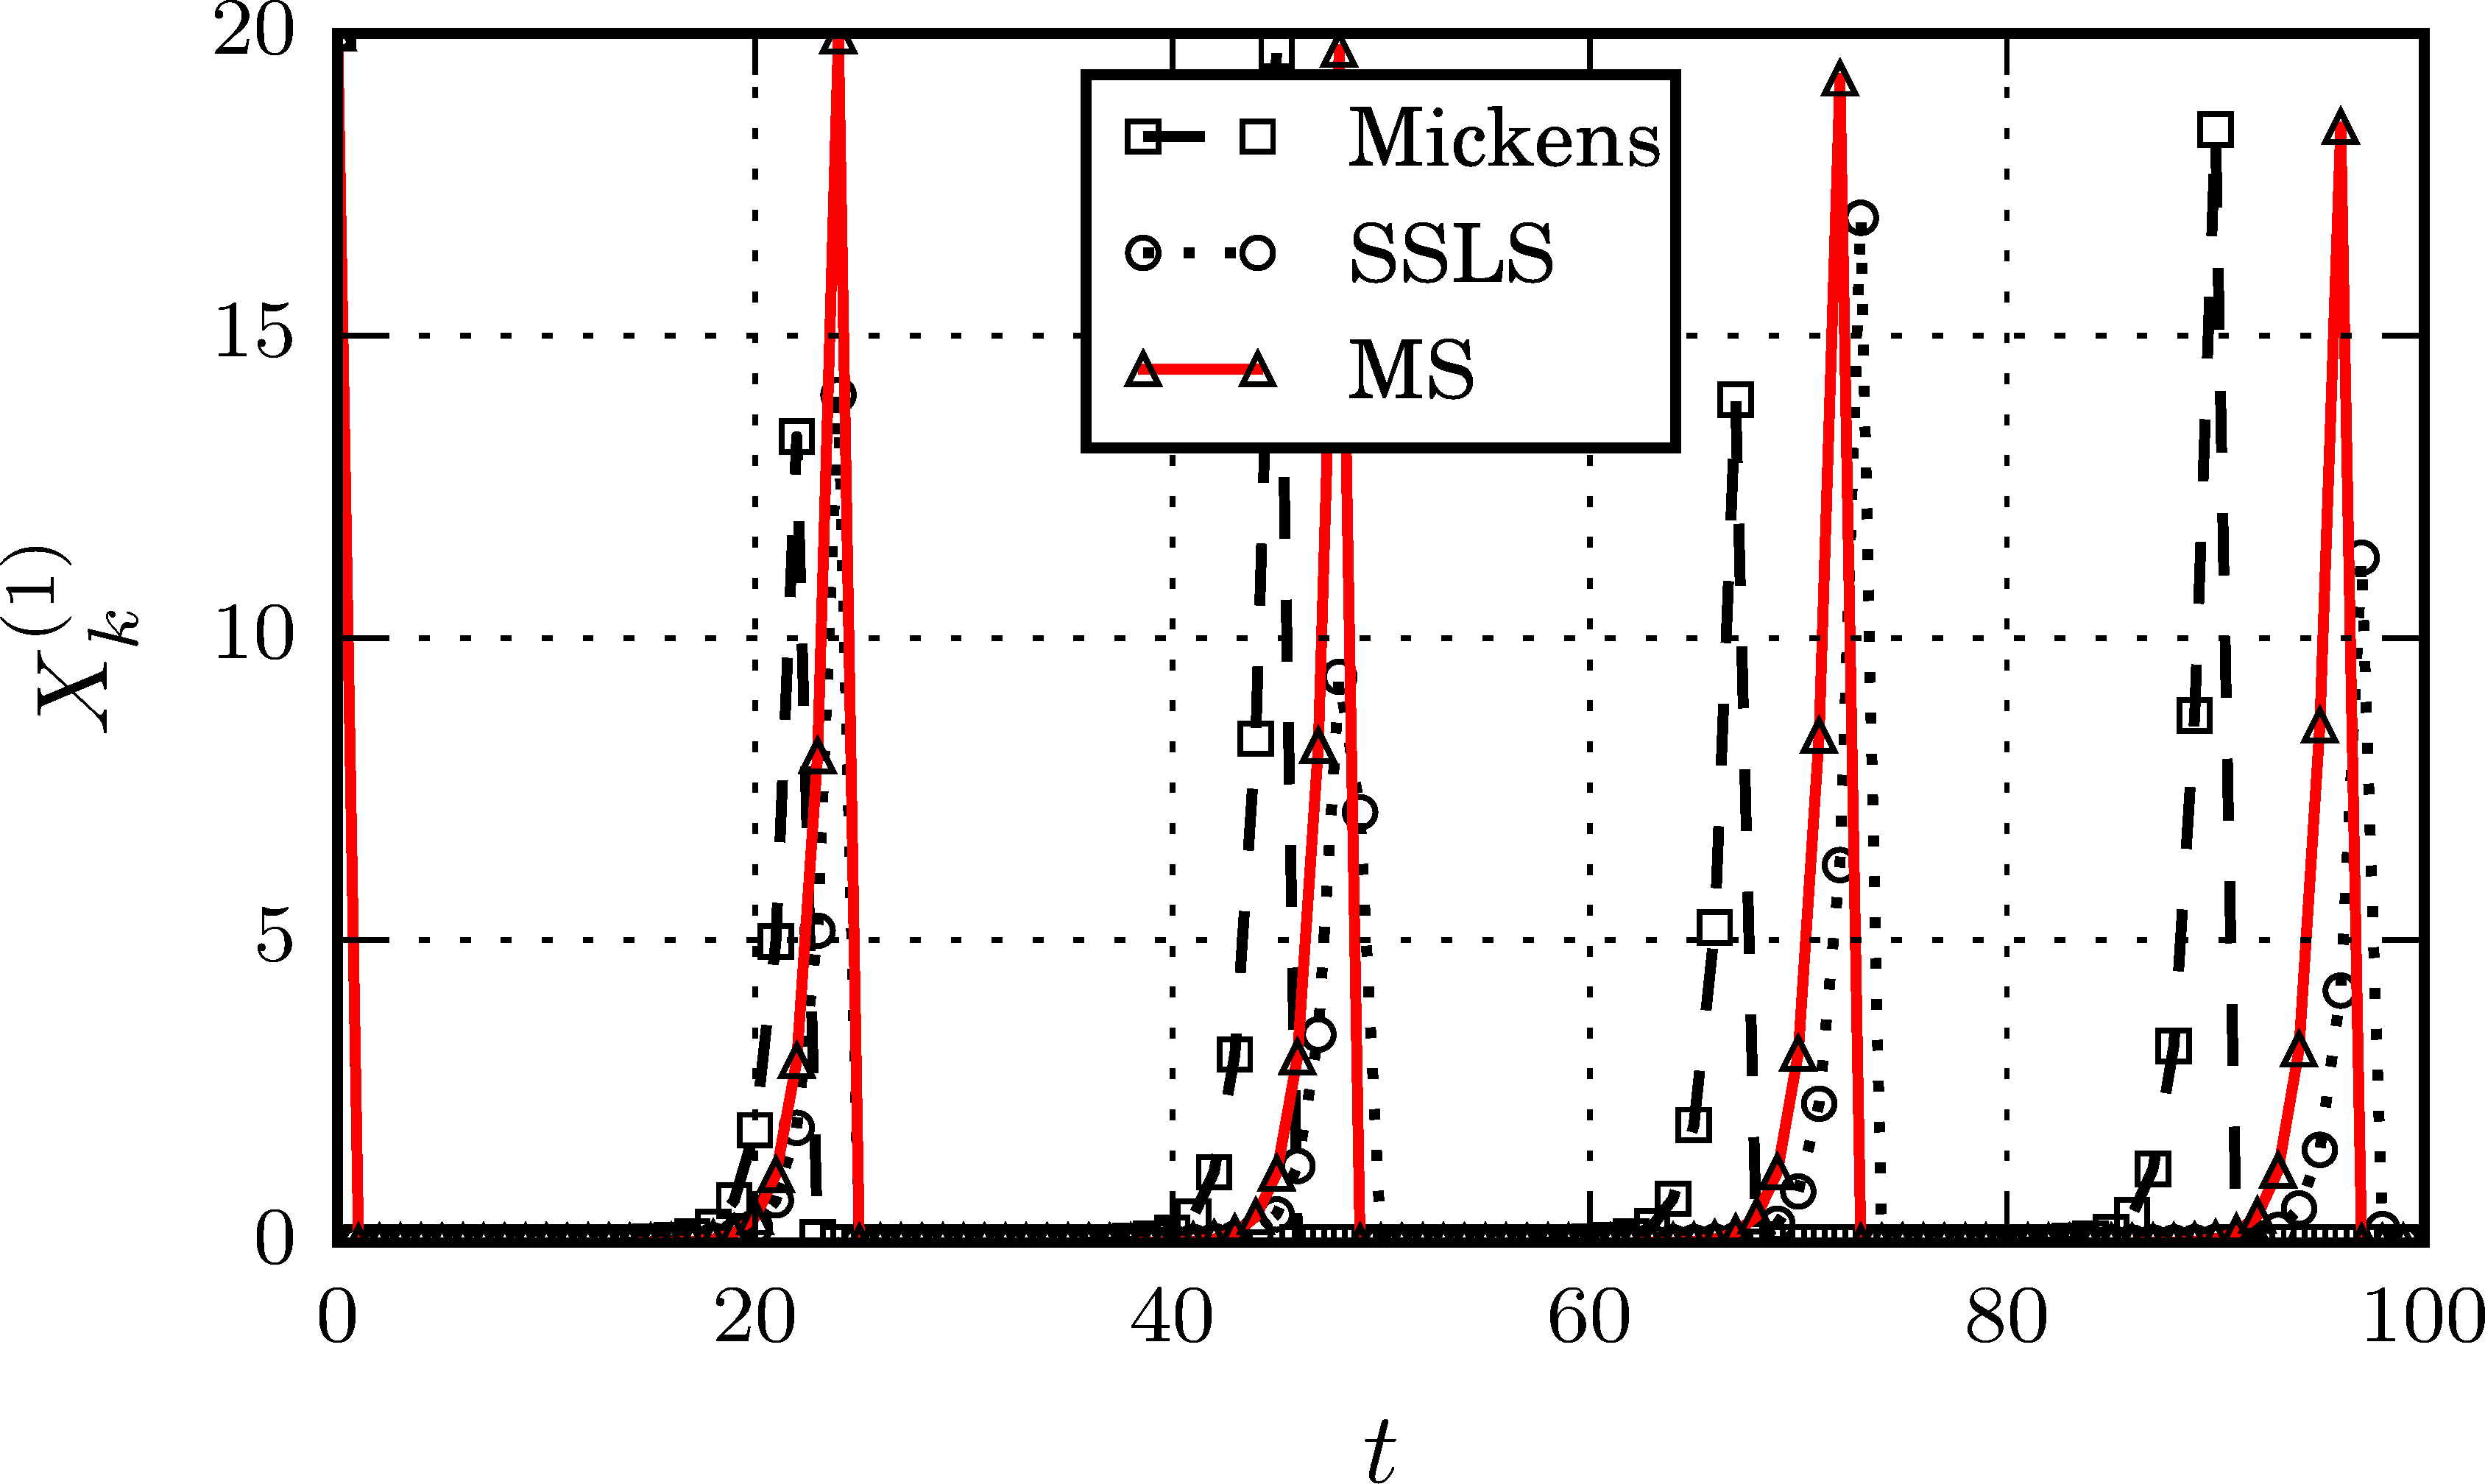
\includegraphics{./papers/paperB/figures/DetX1LotkaVolterraArnold.png}
		\label{subfig:DetX1LotkaVolterraArnold}
		}
	\subfloat[]{
		\centering
		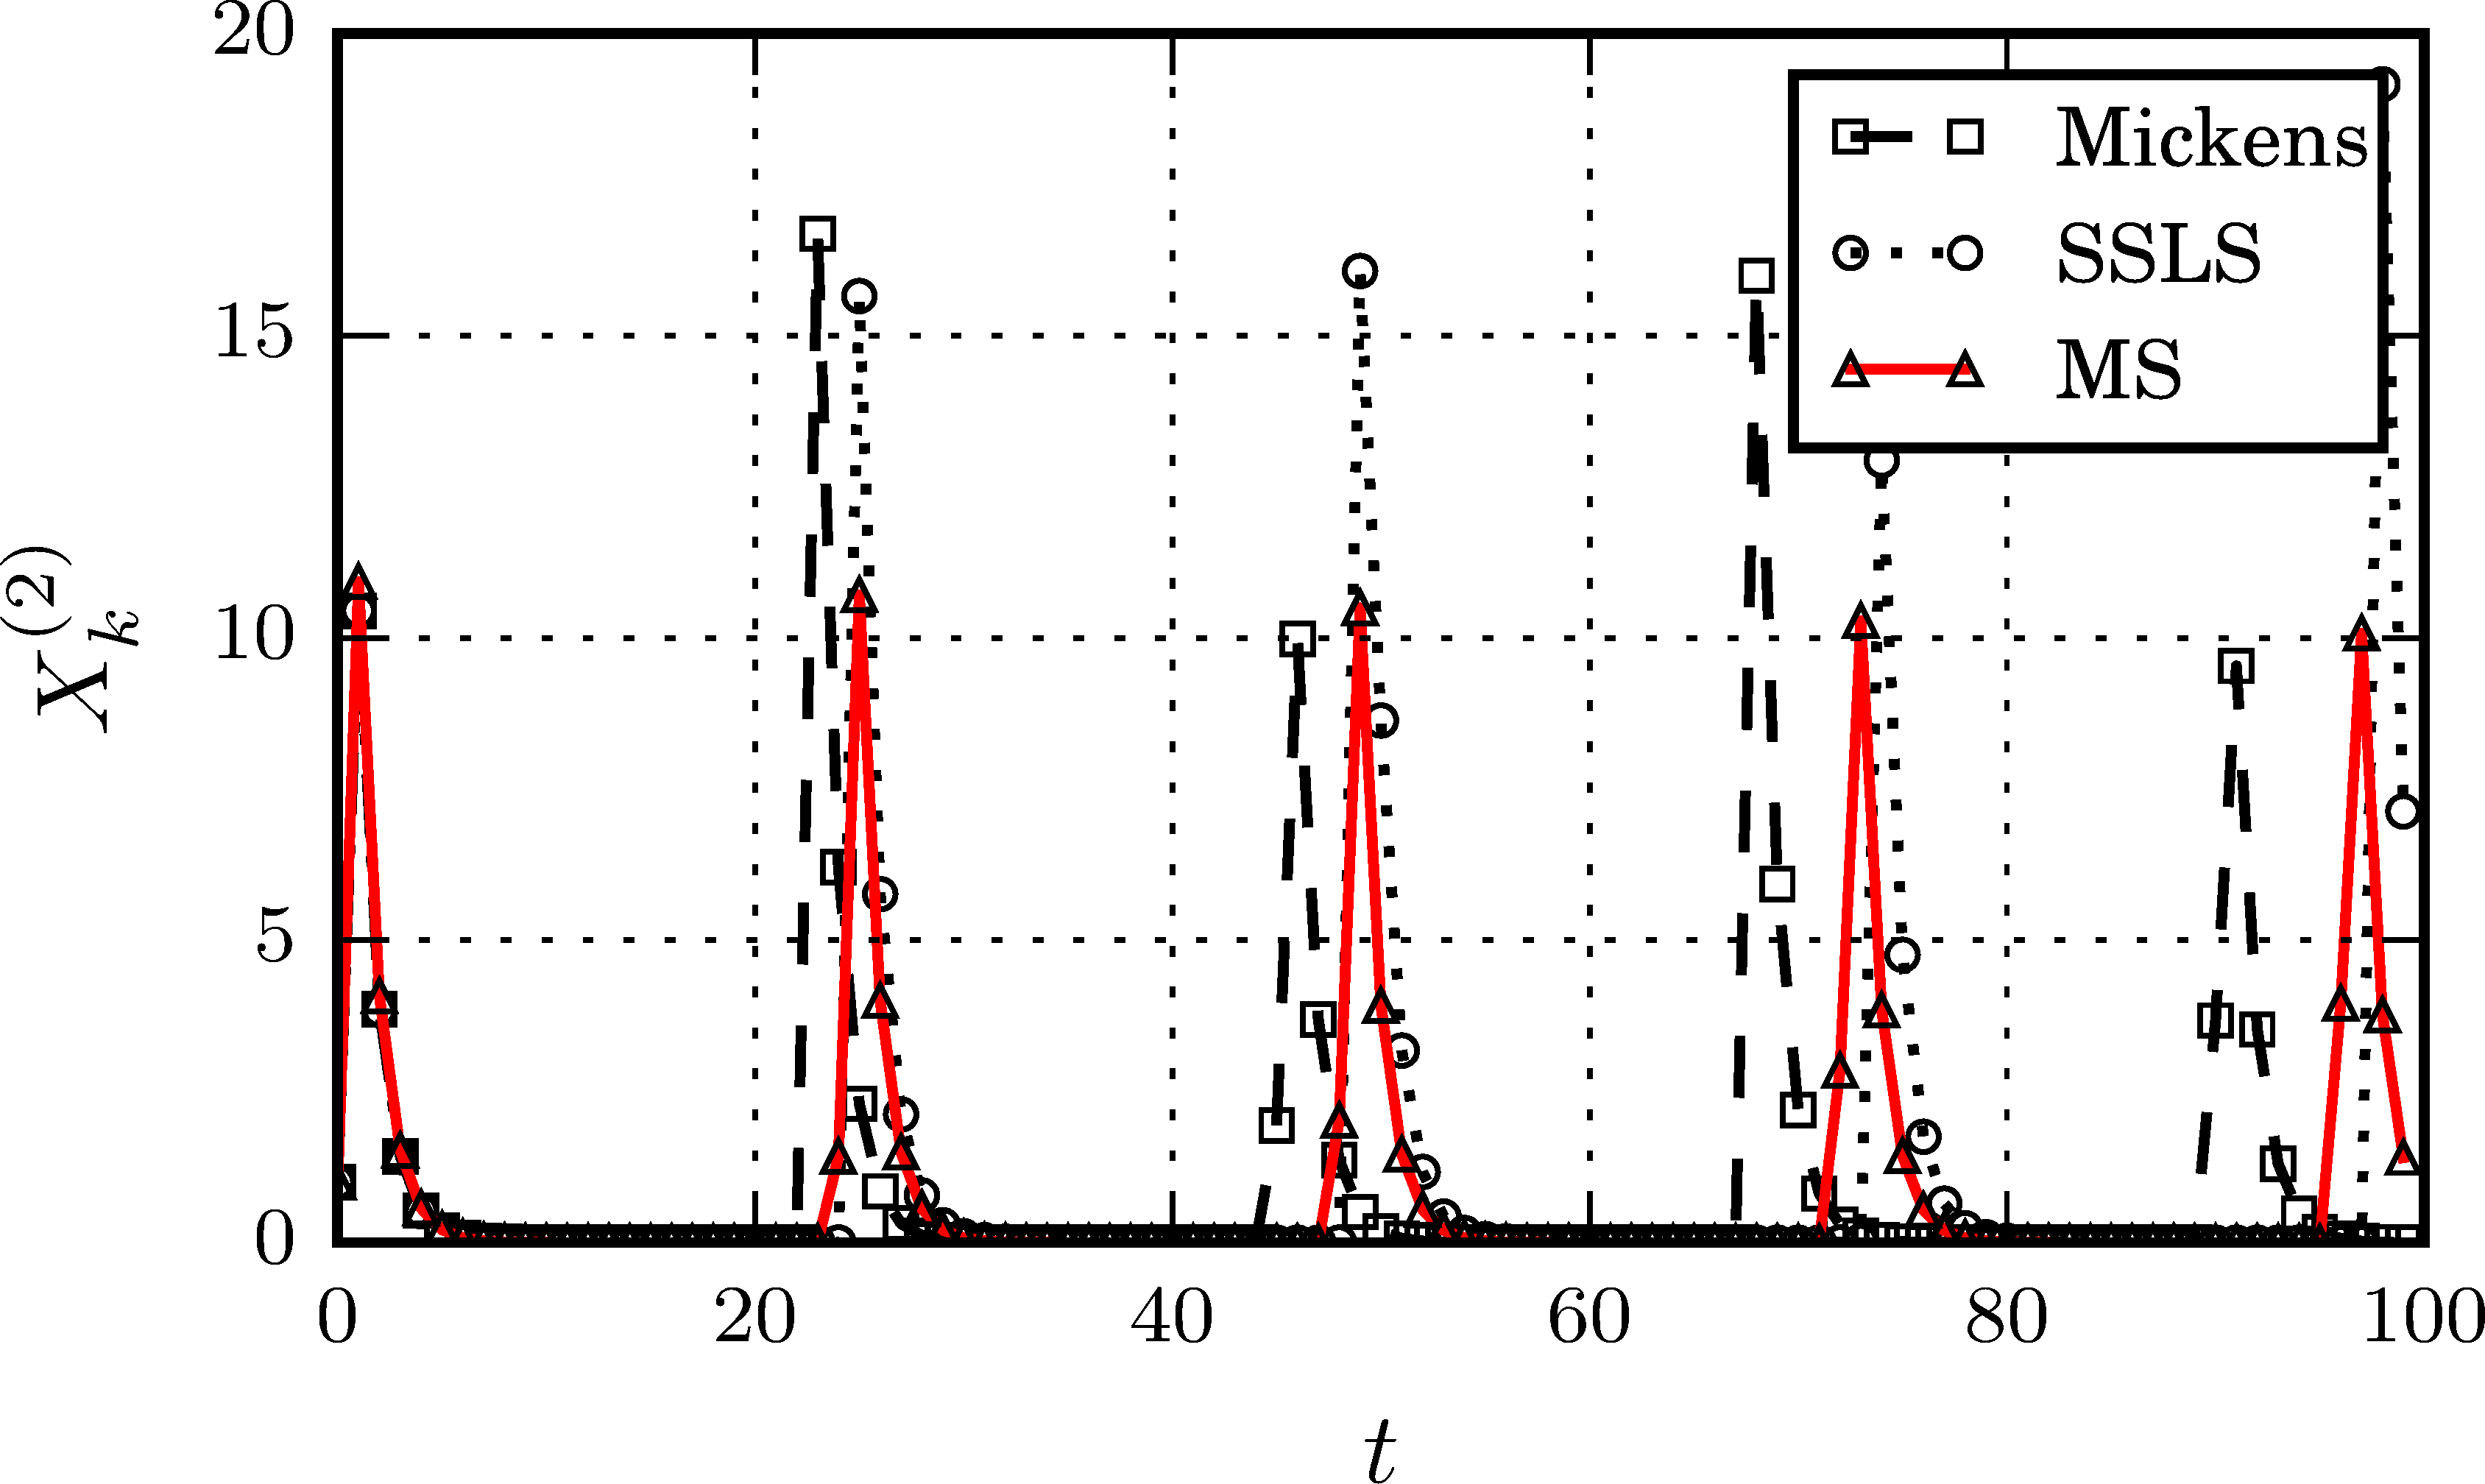
\includegraphics{./papers/paperB/figures/DetX2LotkaVolterraArnold.png}
		\label{subfig:DetX2LotkaVolterraArnold}
	}
	\caption{Likening between the deterministic schemes of Mickens, Serghini and LS for
		the Lotka-Volterra ODE 	\crefrange{eqn:DetLotkaVolterraArnoldA}{eqn:DetLotkaVolterraArnoldB} with 
		$a=1$,
		$b=1$,
		$c=1$,
		%$\sigma=0$,
		$(x_0^{(0)},y_0^{(1)})= (20.0,1.0).$
		$h=\num{.01}$, 
		and over the time interval $[0, 100]$.
	}\label{fig:DeterministicLotkaVolterra}
\end{figure}
\todo{change the legend label MS to Serghini.}
\begin{figure}[tb]
	\centering
	\subfloat[]{
		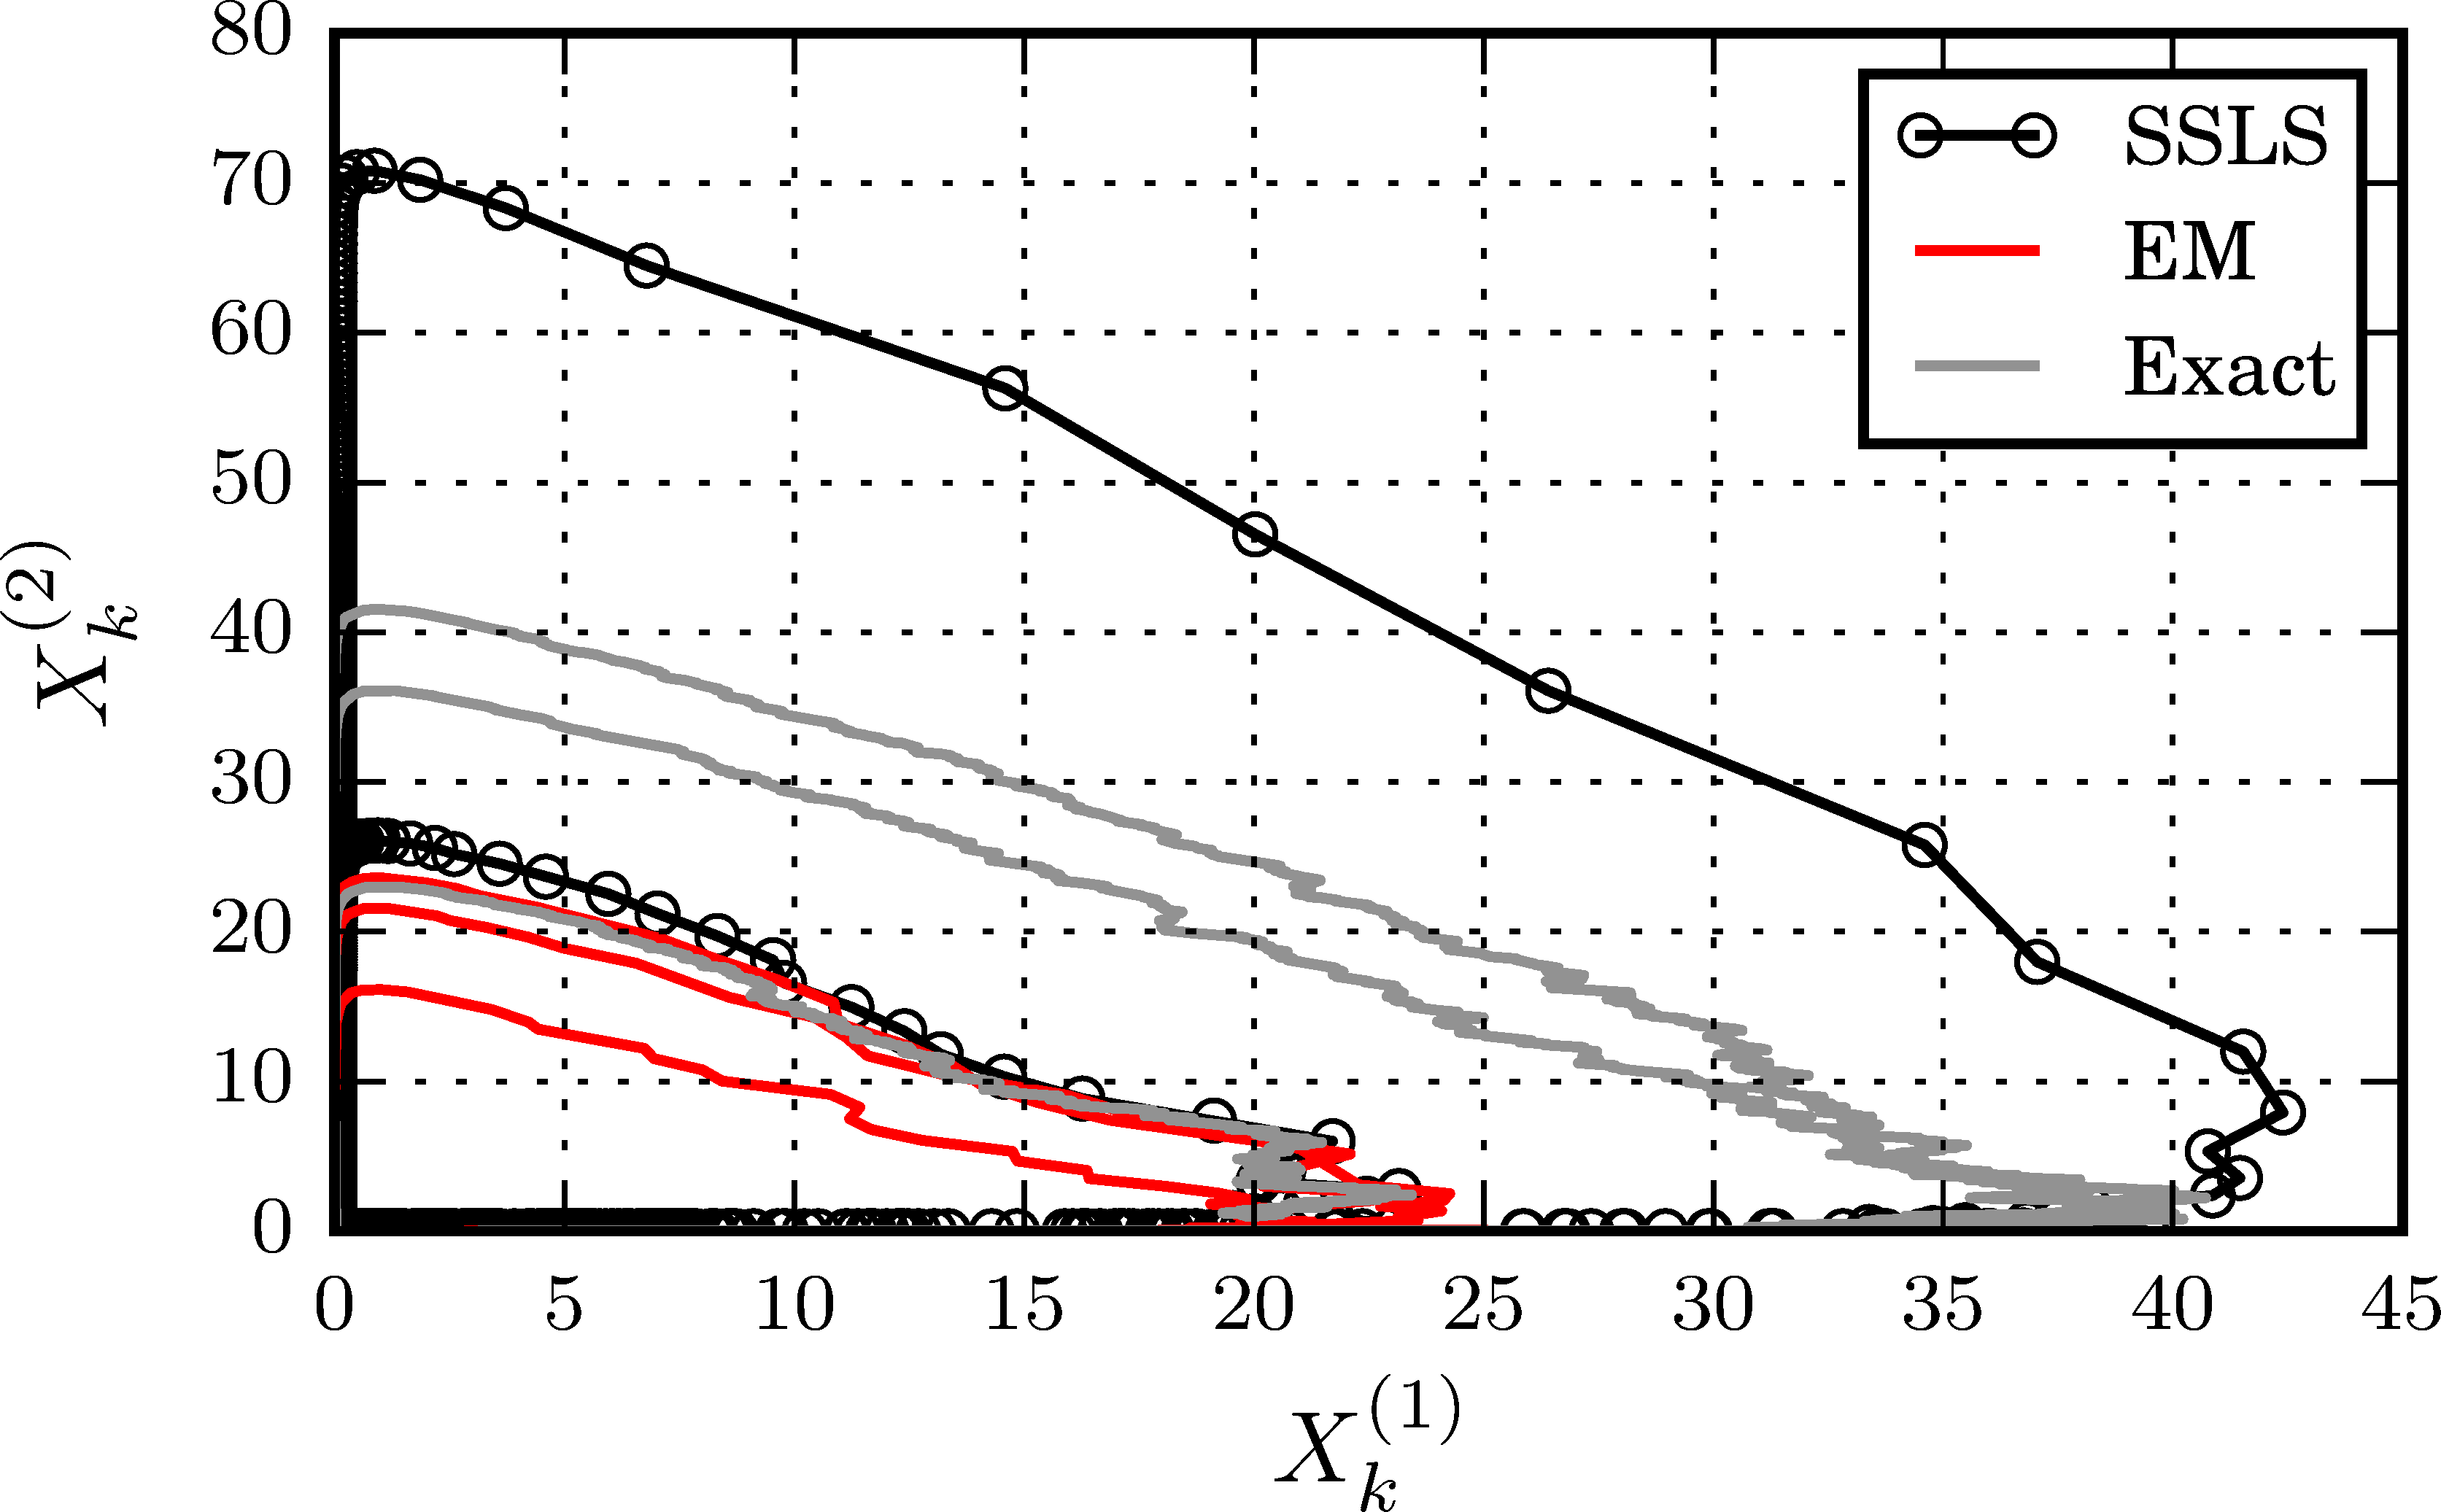
\includegraphics{./papers/paperB/figures/PhasePotraitLotkaVolterraArnold.png}
		\label{subfig:StoPhasePotraitLotkaVolterraArnold}
	}\\
	\subfloat[]{
		\centering
		\includegraphics{./papers/paperB/figures/X1LotkaVolterraArnold.png}
		\label{subfig:StoX1LotkaVolterraArnold}
	}
	\subfloat[]{
		\centering
		\includegraphics{./papers/paperB/figures/X2LotkaVolterraArnold.png}
		\label{subfig:StoX2LotkaVolterraArnold}
	}
	\caption{
		 Likening between the (EM) and  methods for the underlying SDE
		with 
		$a=1$,
		$b=1$,
		$d=1$,
		$\left(X^{1}(0), X^{2}(0)\right) = (20,1)$
		and multiplicative noise intensity $\sigma = \num{0.5}$.
		Here the path labeled with "Exact" means a EM simulation with $h=\num{1e-4}$.
	}\label{fig:LotkaVolterraSDE}
\end{figure}
%
\restoregeometry
\subsection{Environmental Brownian noise suppresses explosions in population dynamics}
	A very important work in stochastic population modeling is \cite{Mao2002}. Here, \citeauthor*{Mao2002}
prove that stochastic environmental noise suppresses the deterministic population explosion, linked to the following SDE
\begin{equation}
	\diag(y_1(t),\dots, y_d(t))
	\left[
	f(y(t))dt + g(y(t))dW(t)
	\right],
\end{equation}
In order to illustrate their results. \citeauthor{Mao2002} report the EM approximation of
\begin{align}
	dy_1(t) &=
		y_1(t) \left[1 - y_1(t) + 2 y_2(t) \right]dt + \varepsilon y_1^2(t) dW_1(t), \label{eqn:MaoPopDynSDE1}\\
	dy_2(t) &=
		y_2(t) \left[1 - 2 y_2(t) + 2 y_1(t)\right]dt + \varepsilon y_2^2(t) dW_2(t) \label{eqn:MaoPopDynSDE2}.
\end{align}
%

	To show that \SM method ()-() preserves this kind of behavior, we perform a numerical realization of this SDE.
In \Cref{fig:MaoPopDynSDE} using the EM and \SM discretizations,  we contrast the explosive deterministic nature of
\crefrange{eqn:MaoPopDynSDE1}{eqn:MaoPopDynSDE2} with its stochastic stabilization.
%
%\begin{align}
%	X_{k+1} &=	\frac{\exp(h a(Y_k)) X_k }{ a(Y_k) + X_k (\exp(h a(y_k)))}
%	\label{eqn:SteklovMatusSDELotka1}\\
%	Y_{k+1} &=	\frac{\exp(2 h b(X_{k+1})) Y_k }{ b(X_{k+1}) + 
%		Y_k( \exp(2h b( X_{k+1})))},
%		\label{eqn:SteklovMatusSDELotka2}
%\end{align}
%and the underlying linearized version \SM.
%
%
%\newgeometry{left=1.75cm, right=1.75cm}
\begin{figure}[h!]
%		\subfloat[]
%		{
%			\centering
%			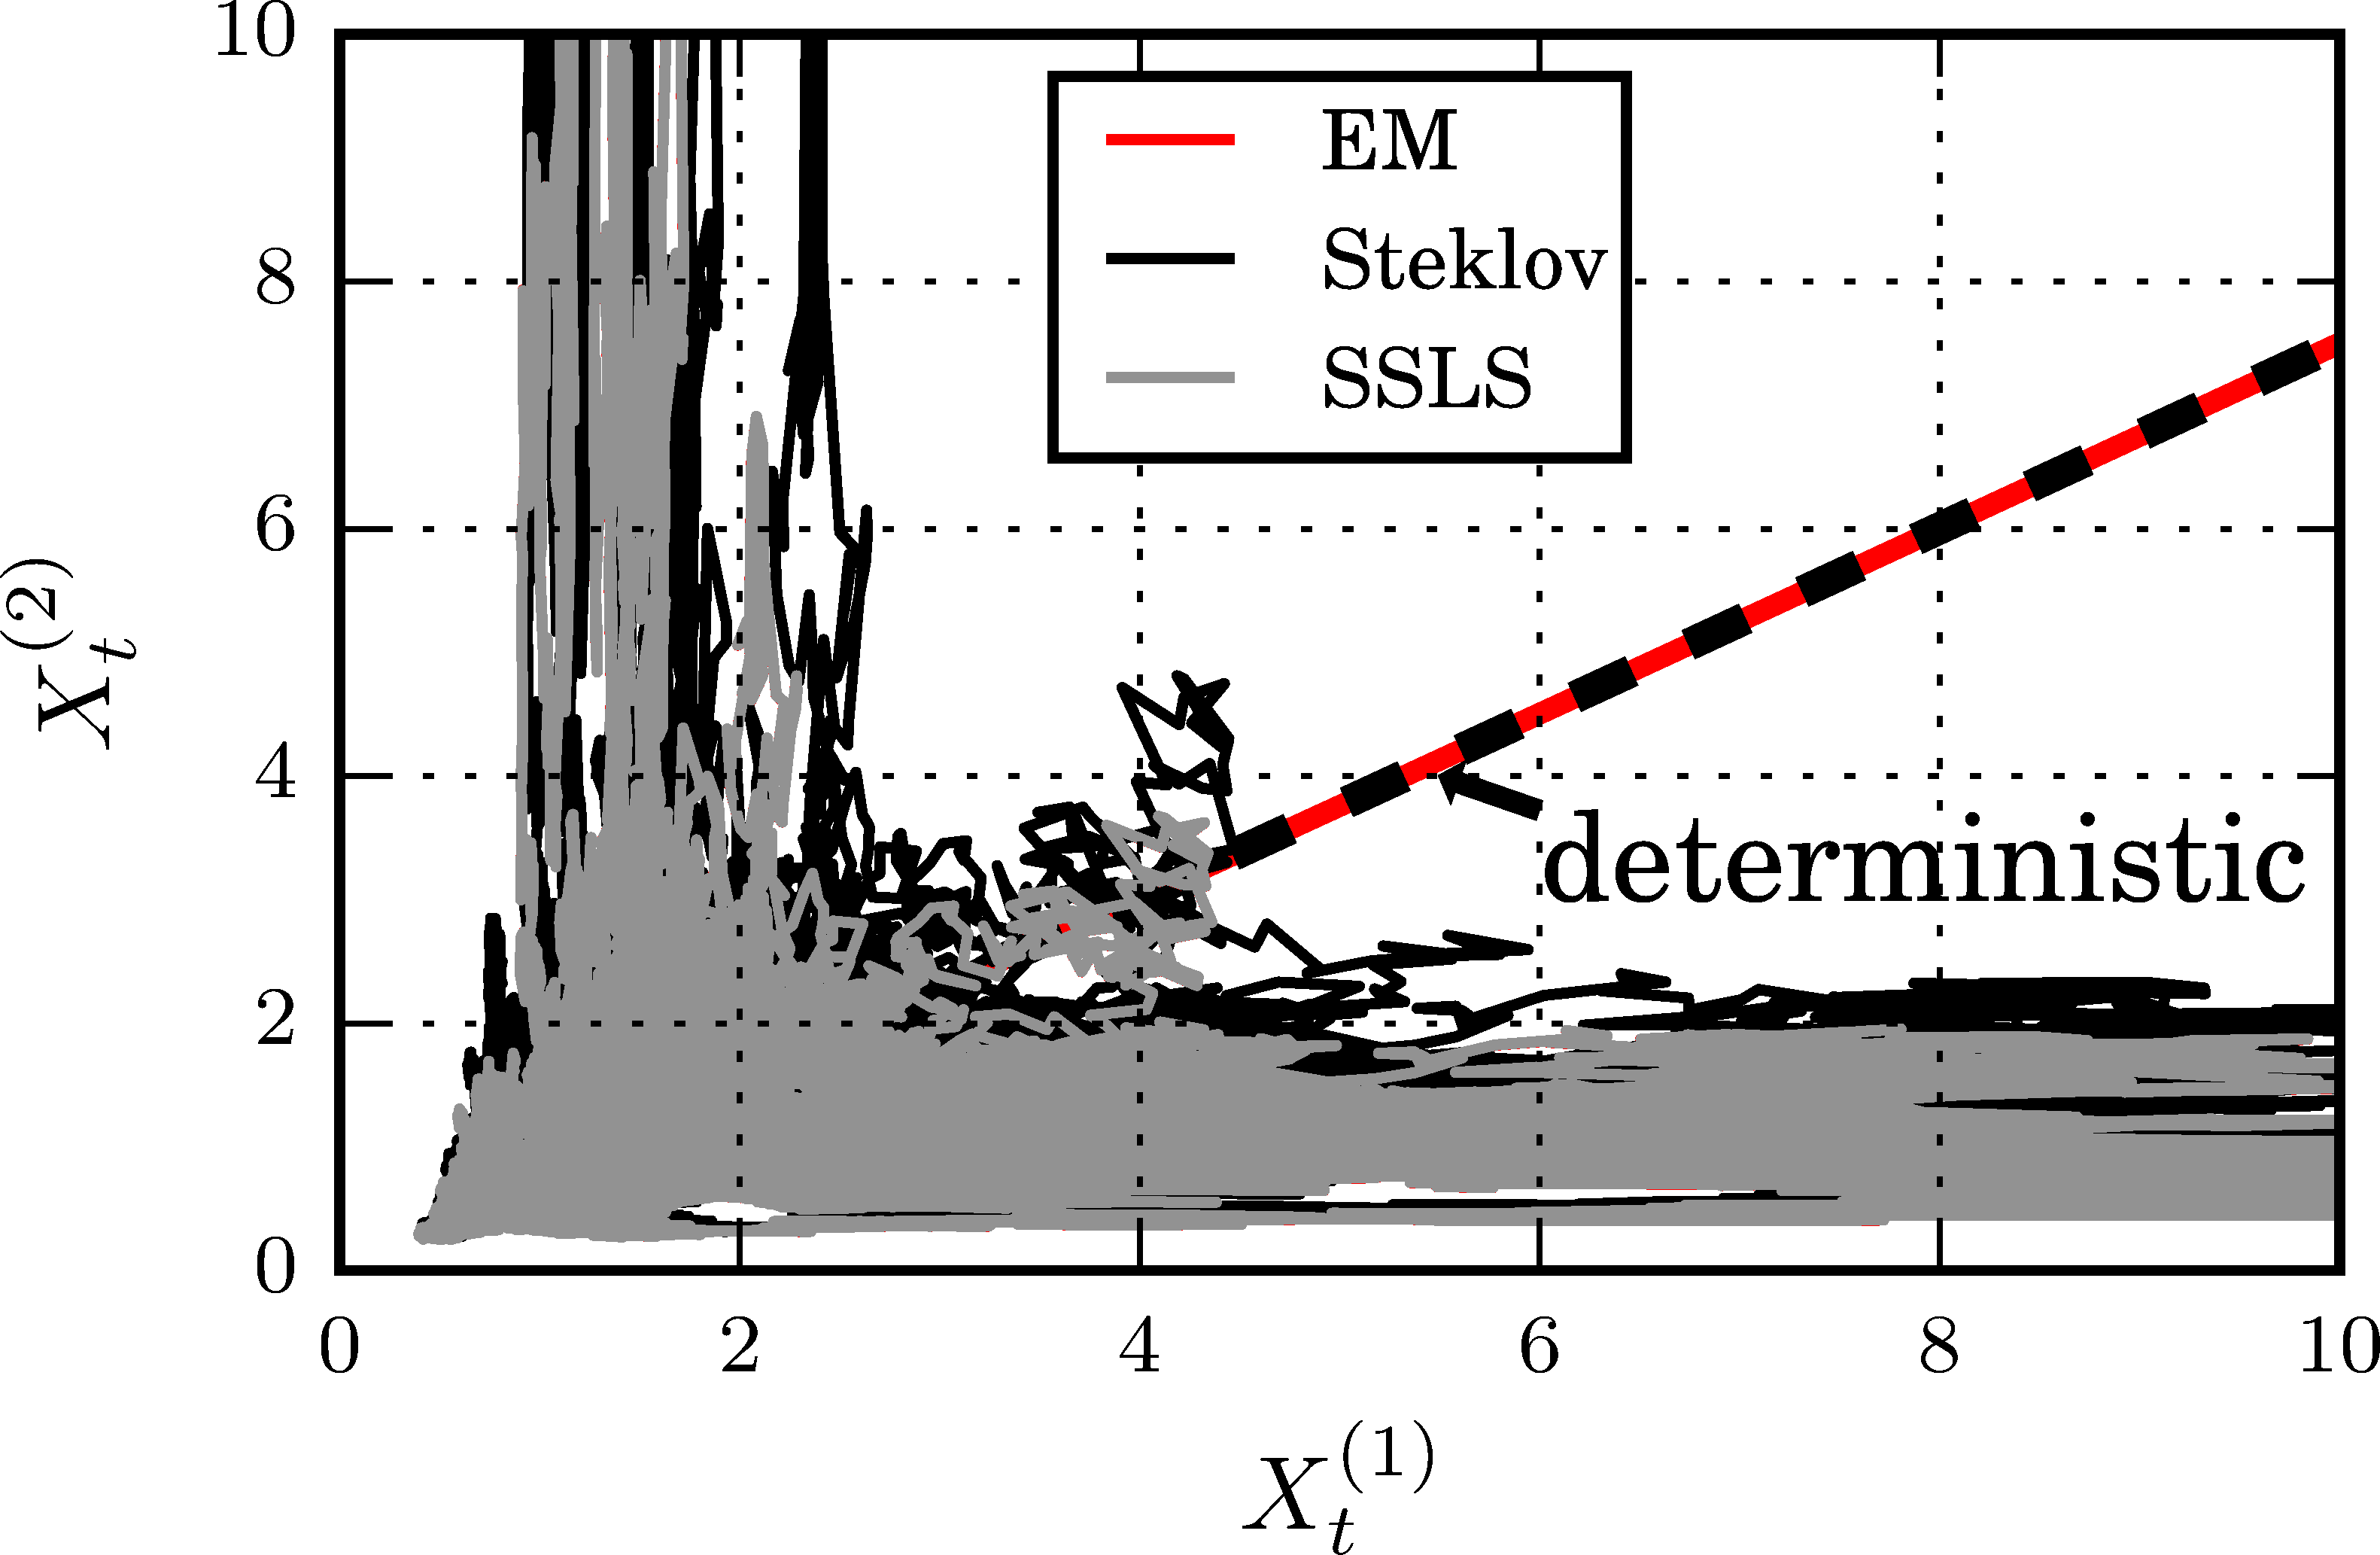
\includegraphics{./papers/paperB/figures/PhasePotraitMao}
%			\label{subfig:StoMaoPopDynPhasePotrait}
%		}\\
	\centering
	\subfloat[]
	{
		\includegraphics{./papers/paperB/figures/StoDetX1Mao}
		\label{subfig:subfig:StoMaoPopDynX1}
	}
	\subfloat[]
	{
		\centering
		\includegraphics{./papers/paperB/figures/StoDetX2Mao}
		\label{subfig:subfig:StoMaoPopDynX2}
	}
	\caption{
		Likening between the numerical solutions of SDE \crefrange{eqn:MaoPopDynSDE1}{eqn:MaoPopDynSDE2} 
		with the EM, Steklov and  \SM methods. We set the noise intensity at $\xi=1$ and fix the initial condition
		to $x(0)=(1, 1)$ over the time interval $T = [0, 10]$, and a step size $h=\num{1e-06}$.
	}
	\label{fig:MaoPopDynSDE}
\end{figure}

\todo{Fix the label into the legends}
\restoregeometry
	\section{Simplified Duffing Van Der Pol Equation}
		This mode is proposal in the classic Kloeden's Book. \\ 
Peter Kloeden \& Eckhard Platen. Numerical Solution of Stochastic Differential Equations.
$$
	\ddot{x}+\dot{x}-(\alpha-x^2)x=\sigma \varepsilon
$$
\begin{align}
	dX_t^{(1)}&= X_t^{(2)} dt \label{eqn:SimDuffingVanDerPolSDE1}\\
	dX_t^{(2)}&=
		\left\{
		X_t^{(1)}
		\left(
			\alpha-(X_t^{(1)})^2
		\right)
		-X_t^{(2)}
	\right\}dt
	+\sigma X_t^{(1)} dW_t \label{eqn:SimDuffingVanDerPolSDE2}
\end{align}
The Steklov Scheme:
\begin{align}
	X^{(1)}_{k+1} &= X^{(1)}_{k} + h X^{(2)}_{k} \notag \\
	X^{(2)}_{k+1} & = a\left(X^{(1)}_{k},X^{(1)}_{k+1}\right)
		\left(
			1 - \exp(-h)
		\right)
		+ \exp(-h) X^{(2)}_{k} + \sigma X^{(1)}_{k} \Delta W_k. \label{eqn:SteklovSimDuffingVanDerPol}\\
		a\left(x, y\right) & = x (\alpha - xy) \notag
\end{align}
In this way also we has been constructed a SSLS for SDE 
\crefrange{eqn:SimDuffingVanDerPolSDE1}{eqn:SimDuffingVanDerPolSDE2} given by
\begin{align}
	X_{k+1}^{(1)} & = X_{k}^{(1)} + h X_{k}^{(2)} \notag\\
	X_{k+1}^{(2)} & = X_{k}^{(2)} 
		\left(
			\exp(-h) - a_2^{(2)}\left(X_{k+1}^{(1)}\right)
		\right) + a_2^{(2)}\left(X_{k+1}^{(1)}\right) 
		+ \sigma X_{k}^{(1)} \Delta W_k
		\label{eqn:SimDuffingVanDerPolSSLS2}\\
		a_2^{(2)}(x) & = x (\alpha - x^2) \notag
\end{align}
In \Cref{fig:SimplifyedDuffingVanDerPolSDE} we present a likening between the EM, two Steklov methods and the Balanced
Implicit scheme (see e.g \cite{Alcock2006}).
\newgeometry{left=1.75cm, bottom=3cm}
\begin{figure}[h!]
	\centering
	\subfloat[]{
		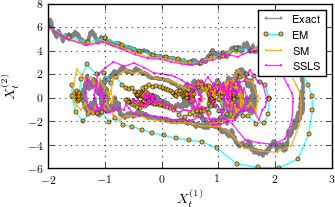
\includegraphics{./papers/paperB/figures/PhasePotraitSimDuffingVanDerPol}
		\label{fig:PhasePotraitSimDuffingVanDerPol}
	}\\
	\subfloat[]{
		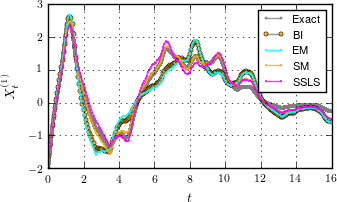
\includegraphics{./papers/paperB/figures/X1SimDuffingVanDerPol.png}
		\label{subfig:X1SimplifiedVanDerPol}
	}
		\subfloat[]{
			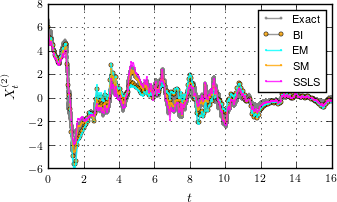
\includegraphics{./papers/paperB/figures/X2SimDuffingVanDerPol.png}
			\label{subfig:X2SimplifiedVanDerPol}
		}
	\caption{Numerical sample paths of SDE \crefrange{eqn:SimDuffingVanDerPolSDE1}{eqn:SimDuffingVanDerPolSDE2}
		with the Euler-Maruyama (EM), Steklov-Mickens (SM) Balanced Implicit(BI) and SSLS methods.
		We set the parameters of the underlying SDE with 
		$\alpha = 1$, 
		$\sigma = 2$,
		$X_0 = (-2, 6)$,
		and fixed the stencil simulation at $h = 2^{-4}$ over the time interval $[0,16]$.
	}
	\label{fig:SimplifyedDuffingVanDerPolSDE}
\end{figure}
\restoregeometry
Gives good results.


	\section{Generalized Van der Pol Oscillator with multiplicative noise}
		This Generalized Van Der Pol oscillator was proposal by Schurz in \cite{Schurz2003}:\\
Schurz, H. General Theorems for Numerical Approximations of Stochastic Processes on the Hilbert 
Space $H_2([0,T], \mu, \mathbb{R}^d)$
\begin{align}
	dX_t^{(1)}	&= X_t^{(2)} dt\\
	dX_t^{(2)}&=
	\left[
		-\omega^2 X_t^{(1)} 
		+\sigma 
		\left(
			1 - \mu_1 \left( X_t^{(1)} \right)^2
			-\mu_2 \left( X_t \right)^2
		\right)
			X_t^{(2)}
	\right]dt
	+\sigma X_t^{(2)} dW_t \label{eqn:GeneralizedVanDerPol1}.
\end{align}
Right now we had constructed the following Linearized Steklov Scheme:
\begin{align}
	a_1^{(2)}(x,y)&:= \gamma (1-\mu_1 x^2 - \mu_2 y^2 ), \qquad
	a_2^{(2)}(x):= -\omega^2 x, \notag \\
	X_{k+1}^{(1)}&=	X_k^{(1)} + h X_k^{(2)}, \\
	X_{k+1}^{(2)}&= 
		\left(
			X_{k}^{(2)}
			+
			\frac{
					a_2
					\left(
						X_{k+1}^{(1)}
					\right)
			}
			{
				a_1^{(2)}
				\left(
					X_{k+1}^{(1)}, X_k^{(2)}
				\right)
			}
		\right)
		\exp
		\left(
			a_1^{(2)}
			\left(
				X_{k+1}^{(1)}, X_k^{(2)}
			\right) h
		\right)
		+\sigma  X_{k}^{(2)} \Delta W_k.
	\notag
\end{align}
This scheme follows almost the same profile of numerical solutions of the Partial Linear
Implicit proposal by Schurz.
\begin{figure}[htb]
\centering
	% GNUPLOT: LaTeX picture with Postscript
\begingroup
  \fontfamily{Times-New-Roman}%
  \selectfont
  \makeatletter
  \providecommand\color[2][]{%
    \GenericError{(gnuplot) \space\space\space\@spaces}{%
      Package color not loaded in conjunction with
      terminal option `colourtext'%
    }{See the gnuplot documentation for explanation.%
    }{Either use 'blacktext' in gnuplot or load the package
      color.sty in LaTeX.}%
    \renewcommand\color[2][]{}%
  }%
  \providecommand\includegraphics[2][]{%
    \GenericError{(gnuplot) \space\space\space\@spaces}{%
      Package graphicx or graphics not loaded%
    }{See the gnuplot documentation for explanation.%
    }{The gnuplot epslatex terminal needs graphicx.sty or graphics.sty.}%
    \renewcommand\includegraphics[2][]{}%
  }%
  \providecommand\rotatebox[2]{#2}%
  \@ifundefined{ifGPcolor}{%
    \newif\ifGPcolor
    \GPcolorfalse
  }{}%
  \@ifundefined{ifGPblacktext}{%
    \newif\ifGPblacktext
    \GPblacktexttrue
  }{}%
  % define a \g@addto@macro without @ in the name:
  \let\gplgaddtomacro\g@addto@macro
  % define empty templates for all commands taking text:
  \gdef\gplbacktext{}%
  \gdef\gplfronttext{}%
  \makeatother
  \ifGPblacktext
    % no textcolor at all
    \def\colorrgb#1{}%
    \def\colorgray#1{}%
  \else
    % gray or color?
    \ifGPcolor
      \def\colorrgb#1{\color[rgb]{#1}}%
      \def\colorgray#1{\color[gray]{#1}}%
      \expandafter\def\csname LTw\endcsname{\color{white}}%
      \expandafter\def\csname LTb\endcsname{\color{black}}%
      \expandafter\def\csname LTa\endcsname{\color{black}}%
      \expandafter\def\csname LT0\endcsname{\color[rgb]{1,0,0}}%
      \expandafter\def\csname LT1\endcsname{\color[rgb]{0,1,0}}%
      \expandafter\def\csname LT2\endcsname{\color[rgb]{0,0,1}}%
      \expandafter\def\csname LT3\endcsname{\color[rgb]{1,0,1}}%
      \expandafter\def\csname LT4\endcsname{\color[rgb]{0,1,1}}%
      \expandafter\def\csname LT5\endcsname{\color[rgb]{1,1,0}}%
      \expandafter\def\csname LT6\endcsname{\color[rgb]{0,0,0}}%
      \expandafter\def\csname LT7\endcsname{\color[rgb]{1,0.3,0}}%
      \expandafter\def\csname LT8\endcsname{\color[rgb]{0.5,0.5,0.5}}%
    \else
      % gray
      \def\colorrgb#1{\color{black}}%
      \def\colorgray#1{\color[gray]{#1}}%
      \expandafter\def\csname LTw\endcsname{\color{white}}%
      \expandafter\def\csname LTb\endcsname{\color{black}}%
      \expandafter\def\csname LTa\endcsname{\color{black}}%
      \expandafter\def\csname LT0\endcsname{\color{black}}%
      \expandafter\def\csname LT1\endcsname{\color{black}}%
      \expandafter\def\csname LT2\endcsname{\color{black}}%
      \expandafter\def\csname LT3\endcsname{\color{black}}%
      \expandafter\def\csname LT4\endcsname{\color{black}}%
      \expandafter\def\csname LT5\endcsname{\color{black}}%
      \expandafter\def\csname LT6\endcsname{\color{black}}%
      \expandafter\def\csname LT7\endcsname{\color{black}}%
      \expandafter\def\csname LT8\endcsname{\color{black}}%
    \fi
  \fi
  \setlength{\unitlength}{0.0500bp}%
  \begin{picture}(7936.00,4902.00)%
    \gplgaddtomacro\gplbacktext{%
      \colorrgb{0.50,0.50,0.50}%
      \put(620,703){\makebox(0,0)[r]{\strut{}-8}}%
      \colorrgb{0.50,0.50,0.50}%
      \put(620,1395){\makebox(0,0)[r]{\strut{}-6}}%
      \colorrgb{0.50,0.50,0.50}%
      \put(620,2087){\makebox(0,0)[r]{\strut{}-4}}%
      \colorrgb{0.50,0.50,0.50}%
      \put(620,2779){\makebox(0,0)[r]{\strut{}-2}}%
      \colorrgb{0.50,0.50,0.50}%
      \put(620,3470){\makebox(0,0)[r]{\strut{} 0}}%
      \colorrgb{0.50,0.50,0.50}%
      \put(620,4162){\makebox(0,0)[r]{\strut{} 2}}%
      \colorrgb{0.50,0.50,0.50}%
      \put(620,4854){\makebox(0,0)[r]{\strut{} 4}}%
      \colorrgb{0.50,0.50,0.50}%
      \put(803,440){\makebox(0,0){\strut{}-1}}%
      \colorrgb{0.50,0.50,0.50}%
      \put(1555,440){\makebox(0,0){\strut{}-0.5}}%
      \colorrgb{0.50,0.50,0.50}%
      \put(2308,440){\makebox(0,0){\strut{} 0}}%
      \colorrgb{0.50,0.50,0.50}%
      \put(3060,440){\makebox(0,0){\strut{} 0.5}}%
      \colorrgb{0.50,0.50,0.50}%
      \put(3813,440){\makebox(0,0){\strut{} 1}}%
      \colorrgb{0.50,0.50,0.50}%
      \put(4565,440){\makebox(0,0){\strut{} 1.5}}%
      \colorrgb{0.50,0.50,0.50}%
      \put(5318,440){\makebox(0,0){\strut{} 2}}%
      \colorrgb{0.50,0.50,0.50}%
      \put(6070,440){\makebox(0,0){\strut{} 2.5}}%
      \colorrgb{0.50,0.50,0.50}%
      \put(6823,440){\makebox(0,0){\strut{} 3}}%
      \colorrgb{0.50,0.50,0.50}%
      \put(7575,440){\makebox(0,0){\strut{} 3.5}}%
      \csname LTb\endcsname%
      \put(160,2778){\rotatebox{-270}{\makebox(0,0){\strut{}$X^{(2)}_k$}}}%
      \put(4189,140){\makebox(0,0){\strut{}$X^{(1)}_k$}}%
    }%
    \gplgaddtomacro\gplfronttext{%
      \csname LTb\endcsname%
      \put(6672,4691){\makebox(0,0)[r]{\strut{}Exact}}%
      \csname LTb\endcsname%
      \put(6672,4491){\makebox(0,0)[r]{\strut{}SSLS h =.001}}%
      \csname LTb\endcsname%
      \put(6672,4291){\makebox(0,0)[r]{\strut{}PLIE h =.001}}%
    }%
    \gplbacktext
    \put(0,0){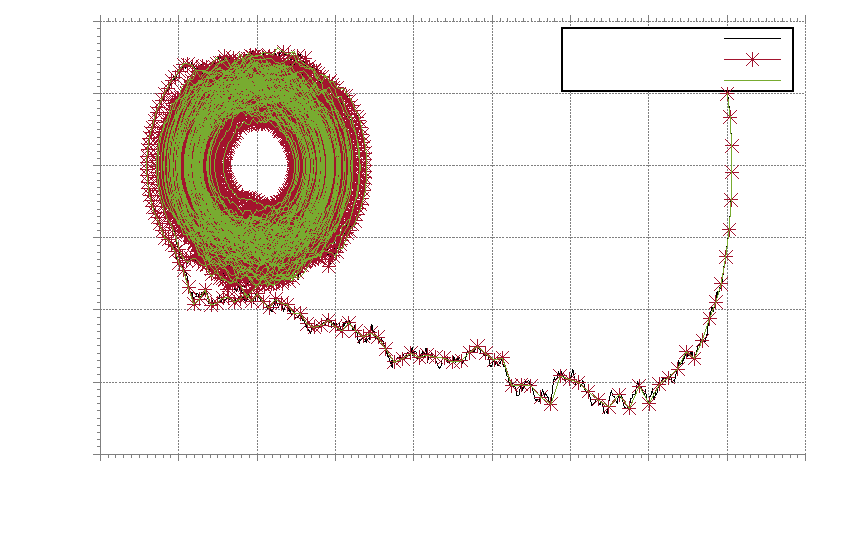
\includegraphics{./papers/paperB/figures/PhasePotrait}}%
    \gplfronttext
  \end{picture}%
\endgroup

	\caption{'Typical' trajectory of SDE \eqref{eqn:GeneralizedVanDerPol1}
		with 
		$\omega = \num{5}$, 
		$\gamma = \num{1.0}$,
		$\mu_1 = \num{0.05}$,
		$\mu_2 = \num{0.25}$,
		$\sigma = \num{0.5}$,
		$X_0 = (\num{3}, \num{2})^T$
		and discretized with the SSLS and PLIE schemes. Here exact means a discretization with the EM 
		scheme using a step size of $h=\num{1e-4}$.
	}
\label{fig:GenVanDerPolPhasePotrait}
\end{figure}




















































	\section{Stochastic Lorenz Equation}
		
	We want to compare the performance of the Steklov Scheme with simulations of the Stochastic
Lorenz System proposal in \cite{Keller1996}.
H. Keller. Attractors and bifurcations of the stochastic Lorenz system.
\begin{align}
	du &= (-Au - B(u) + f)dt +C(u)dW(t) \notag\\
	A & = 
	\begin{bmatrix}
		\sigma	&-\sigma	&0\\
		\sigma	&1			&0\\
		0		&0			&\beta
	\end{bmatrix}, 
	\qquad
	B(u) = 
	\begin{bmatrix}
		0\\
		xz\\
		-xy
	\end{bmatrix},
	\qquad
	f=
	\begin{bmatrix}
		0\\
		0\\
		-\beta(r+\sigma)
	\end{bmatrix} \label{eqn:LorenzSDE}\\
	C(u) &: \mathbb{R}^3 \to \mathbb{M}_{3 \times m}(\mathbb{R}), \qquad
	\|C(u)\|^2 = \Tr\left(C(u)C(u)^T\right)\leq K^2(1+ \|u\|^2).
	\notag
\end{align}
The simulations was performed with $C(u)=\sqrt{q}u$.
The following SSLS scheme gives good results.
\begin{align}
	a_1(y) &= \sigma y, \qquad a_2(x,z) = -x (\sigma +z) \qquad 
	a_3(x,y) = x y -\beta(\sigma +r) \notag\\
	X_{k+1} &= \exp(-\sigma h) X_{k}
		+\frac{a_1(Y_k)}{\sigma}
		(1-\exp(-\sigma h)), \notag\\
	Y_{k+1} &= a_2(X_{k+1},Z_{k}) (1-\exp(-h))
		+Y_k \exp(-h), \label{eqn:LorenzSSLS}\\
	Z_{k+1} &= \frac{a_3(X_{k+1}, Y_{k+1})}{\beta} (1- \exp(-\beta h))
		+Z_{k} \exp(-\beta h), \notag\\
	u_{k+1} &= (X_{k+1},Y_{k+1},Z_{k+1})^T + \sqrt{q} \Delta W_k (X_{k},Y_{k},Z_{k})^T.
	\notag
\end{align}

	In \Cref{fig:LorenzPaths} we present bought, deterministic and stochastic paths of Lorenz
SDE \Cref{eqn:LorenzSDE} produced by the \SM scheme \eqref{eqn:LorenzSSLS}. Also, in order to compare
the performance of the underlying scheme, in \Cref{fig:LorenzNumericalDis} we show the associated 
distribution of the last \num{1000} steps generated with the EM and \SM methods.
%
\begin{figure}[h!]
	\subfloat[Deterministic $q=\num{0}$.]{
		\centering
		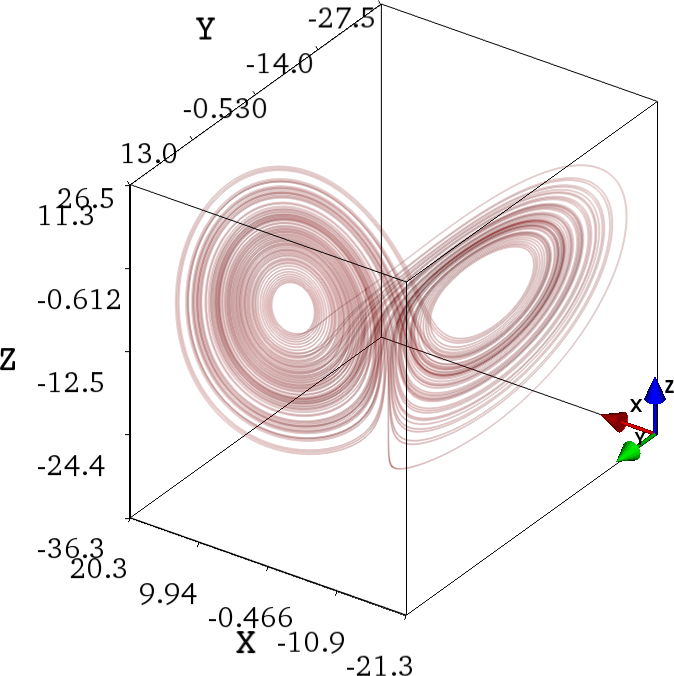
\includegraphics[width=0.45\linewidth]{./papers/paperB/figures/SDELorenz1.png}
		}
		\subfloat[Noise intensity $q = \num{0.3}$]{
			\centering
			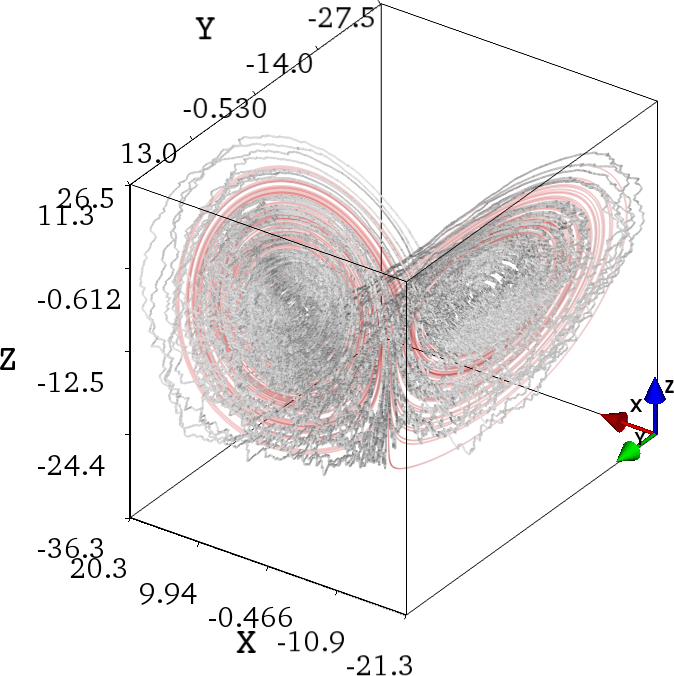
\includegraphics[width=0.45\linewidth]{./papers/paperB/figures/SDELorenz2.png}
		}
	\caption{Simulated paths of the Lorentz SDE \eqref{eqn:LorenzSDE} using the SSLS scheme
		\eqref{eqn:LorenzSSLS}. At the left the color red denotes the deterministic path with 
		$T = 100.0$,
		$h = \num{1e-06}$,
		$\sigma = \num{10.0}$,
		$\beta = \num{2.67}$,
		$\rho = \num{28.0}$,
		$U_0 = [\num{2.0}, \num{2.0}, \num{-9.0}]$.
		On the right, the gray color denotes the resulting path with same parameter and multiplicative 
		intensity $q = \num{0.3}$ noise.
	}\label{fig:LorenzPaths}
\end{figure}
\newgeometry{left=1.75cm, top=2cm, bottom=2cm}
\begin{figure}[htb]
	\centering
	\subfloat[EM $h=\num{1e-4}$.]{
		\includegraphics[width=0.4\textwidth]{./papers/paperB/figures/Histogram/EMDistributionh1.png}
		\label{subfig:EMDistLorenzSDE}
	}
	\subfloat[SSLS $h = \num{1e-4}$.]{
		\includegraphics[width=0.4\textwidth]{./papers/paperB/figures/Histogram/SSDistributionh1.png}
		\label{subfig:SSLSDistLorenzSDE}
	}\\
	\subfloat[EM $h=\num{1e-3}$.]{
		\includegraphics[width=0.4\textwidth]{./papers/paperB/figures/Histogram/EMDistributionh2.png}
		\label{subfig:EMDist2LorenzSDE}
	}
	\subfloat[SSLS $h=\num{1e-3}$.]{
		\includegraphics[width=0.4\textwidth]{./papers/paperB/figures/Histogram/SSDistributionh2.png}
		\label{subfig:SSLSDist2LorenzSDE}
	}\\
	\subfloat[EM $h=\num{1e-2}$.]{
		\includegraphics[width=0.4\textwidth]{./papers/paperB/figures/Histogram/EMDistributionh3.png}
		\label{subfig:EMDist3LorenzSDE}
	}
	\subfloat[SSLS $h=\num{1e-2}$.]{
		\includegraphics[width=0.4\textwidth]{./papers/paperB/figures/Histogram/SSDistributionh3.png}
		\label{subfig:SSLSDist3LorenzSDE}
	}
	\caption{Numerical distribution of the last \num{1000} time $h$ steps of the Lorenz SDE.
	\cref{eqn:LorenzSDE}}
	\label{fig:LorenzNumericalDis}
\end{figure}
\restoregeometry


	\section{Stochastic AIDS}
		
	The HIV internal dynamics is the interaction between the HIV-1 virus and the immune system. 
\citeauthor*{Dalal2008} in \cite{Dalal2008} propose a compartmental stochastic model, which capture the interaction 
between CD-4 for cells and HVI-1 virus. They perturbed  with noise the per capita rate parameters of the three kind of 
populations described by
\begin{align}\label{eqn:HIVDynamics}
	\frac{dy_1(t)}{dt} &=
		\left(
			\lambda -\delta y_1(t) - (1 - \gamma) \beta y_1(t) y_3(t)
		\right),
		\notag \\
	\frac{dy_2(t)}{dt} &= 
		\left(
			(1- \gamma) \beta y_1(t) y_3(t) - a y_2(t) 
		\right),
	\\
	\frac{dy_3(t)}{dt} & = 
		\left(
			(1 - \eta) N a y_2(t) 
			-u y_3(t)
			-(1 - \gamma ) \beta y_1(t) y_3(t) 
		\right).
	\notag
\end{align}
Where:
\begin{table}[h!]
	\begin{center}
	\begin{tabular}{rl}
		$y_1(t)$ &				is the concentration of uninfected cells;\\ 
		$y_2(t)$ &				is the concentration of infected cells; \\
		$y_3(t)$ &				is the concentration of virus particles;\\
		$(1 - \gamma)$ &	is the reverse transcriptase inhibitor drug effect;\\
		$(1 -\eta)$ &			is the protease inhibitor drug effect; \\
		$\lambda$ &				is the total rate of production of healthy cells per unit time;\\
		$\delta$ &				is the per capita death rate of healthy cells;\\
		$\beta$ &					is the transmission coefficient between uninfected cells and infective virus particles;\\
		$a$ & 						is the per capita death rate of infected cells;\\
		$N$ &							is the average number of infective virus particles produced by an infected\\ 
				&							cell in the absence of the Highly Active Antiretroviral Treatment (HAART)\\
				&							during its entire infectious lifetime; \\
		$u$&							is the per capita death rate of infective virus particles.
	\end{tabular}
	\end{center}
\end{table}

	Because rates of death for both, CD-4 cells and HIV-1 virus are affected by great amount of biological complex 
mechanisms, the authors introduce randomness into the model by replacing the parameters $\delta$, $a$, and $u$ by
$\delta \to \delta+ \sigma_1 dW^{(1)}_t$,
$a \to a + \sigma_2 dW^{(1)}_t$, and
$u \to u + \sigma_2 dW^{(2)}_t$,
where $W^{(1)}_t$, $W^{(2)}_t$ are independent Brownian motions with intensities $\sigma_1$, $\sigma_2$.
They obtain the following system of stochastic differential equations
\begin{align}\label{eqn:StochasticHIVDynamics}
	dy_1(t) &=
		\left(
			\lambda -\delta y_1(t) - (1 - \gamma) \beta y_1(t) y_3(t)
		\right)dt,
		-\sigma_1 y_1(t) dW^{(1)}_t, 
		\notag \\
	dy_2(t) &= 
		\left(
			(1- \gamma) \beta y_1(t) y_3(t) - a y_2(t) 
		\right)dt,
		-\sigma_1 y_2(t) dW^{(1)}_t, 
	\\
	dy_3(t) & = 
	\left(
		(1 - \eta) N a y_2(t) 
		-u y_3(t)
		-(1 - \gamma ) \beta y_1(t) y_3(t) 
	\right)dt
	- \sigma_2 y_3(t) dW^{(2)}_t.
	\notag
\end{align}

	\citeauthor{Dalal2008} give suitable conditions to assure that  the number of infected cells and virus particles tend
asymptotically to zero almost surely \cite[Thm. 5.1]{Dalal2008}. They support their analytical results by the 
simulation of SDE 
\eqref{eqn:StochasticHIVDynamics}. All the parameters values that they used, have been taken from published 
literature \cite{Bonhoeffer1997, Callaway2002, Nelson2000, Nowak1997}.

	Using the following \SM scheme
\begin{align}\label{eqn:SteklovSchemMaoAdis2}
	X^{(j)}_{k+1}
			&=
			\left(
				X_k^{(j)} + 
				\frac{b_j }{a_j}
			\right) 
			\exp\left(
					a_j h
				\right) - \frac{b_j}{a_j}
		+ g^{(j)}(X_k) \Delta W^{(j)}_k, \qquad j \in \{1,2,3\} \notag 
		\\
	g^{(1)}(X_k) &=- \sigma_1 X_{k}^{(1)},  \qquad
	g^{(2)}(X_k)= - \sigma_1 X_{k}^{(2)}, \qquad
	g^{(3)}(X_k)= - \sigma_2 X_{k}^{(3)}, \notag
\end{align}
\begin{alignat}{2}%\label{eqn:SteklovHIVDynamicsCoef}	
	a_{1} &= 
		-\left(
			\delta + (1 - \gamma) \beta X_{k}^{(3)}
		\right),
	& \qquad
	b_1 &= \lambda, \notag
	\\
	a_{2} &= -a,
	& \qquad
	b_2 &=
		(1-\gamma) \beta X_{k+1}^{(1)} X_{k}^{(3)}, 
\\
	a_{3} &= 
		-
	\left(
			u + (1- \gamma) \beta X_{k+1}^{(1)}
		\right),
	& \qquad
	b_{3} &= 
		\left(
			1 - \eta 
		\right)
		N a X_{k+1}^{(3)}, \notag
\end{alignat}
we contrast the approximations of SDE \eqref{eqn:StochasticHIVDynamics} with the corresponding EM method.
In \Cref{fig:StochasticHIVDynamicsPaths} utilizing a step-size $h=\num{0.5}$, we observe how the EM method diverge,
while the \SM obeys the EM numerical realization of the solution with a very small ($h=\num{0.0005}$) step-size.
\begin{figure}[htb]
	\begin{center}
		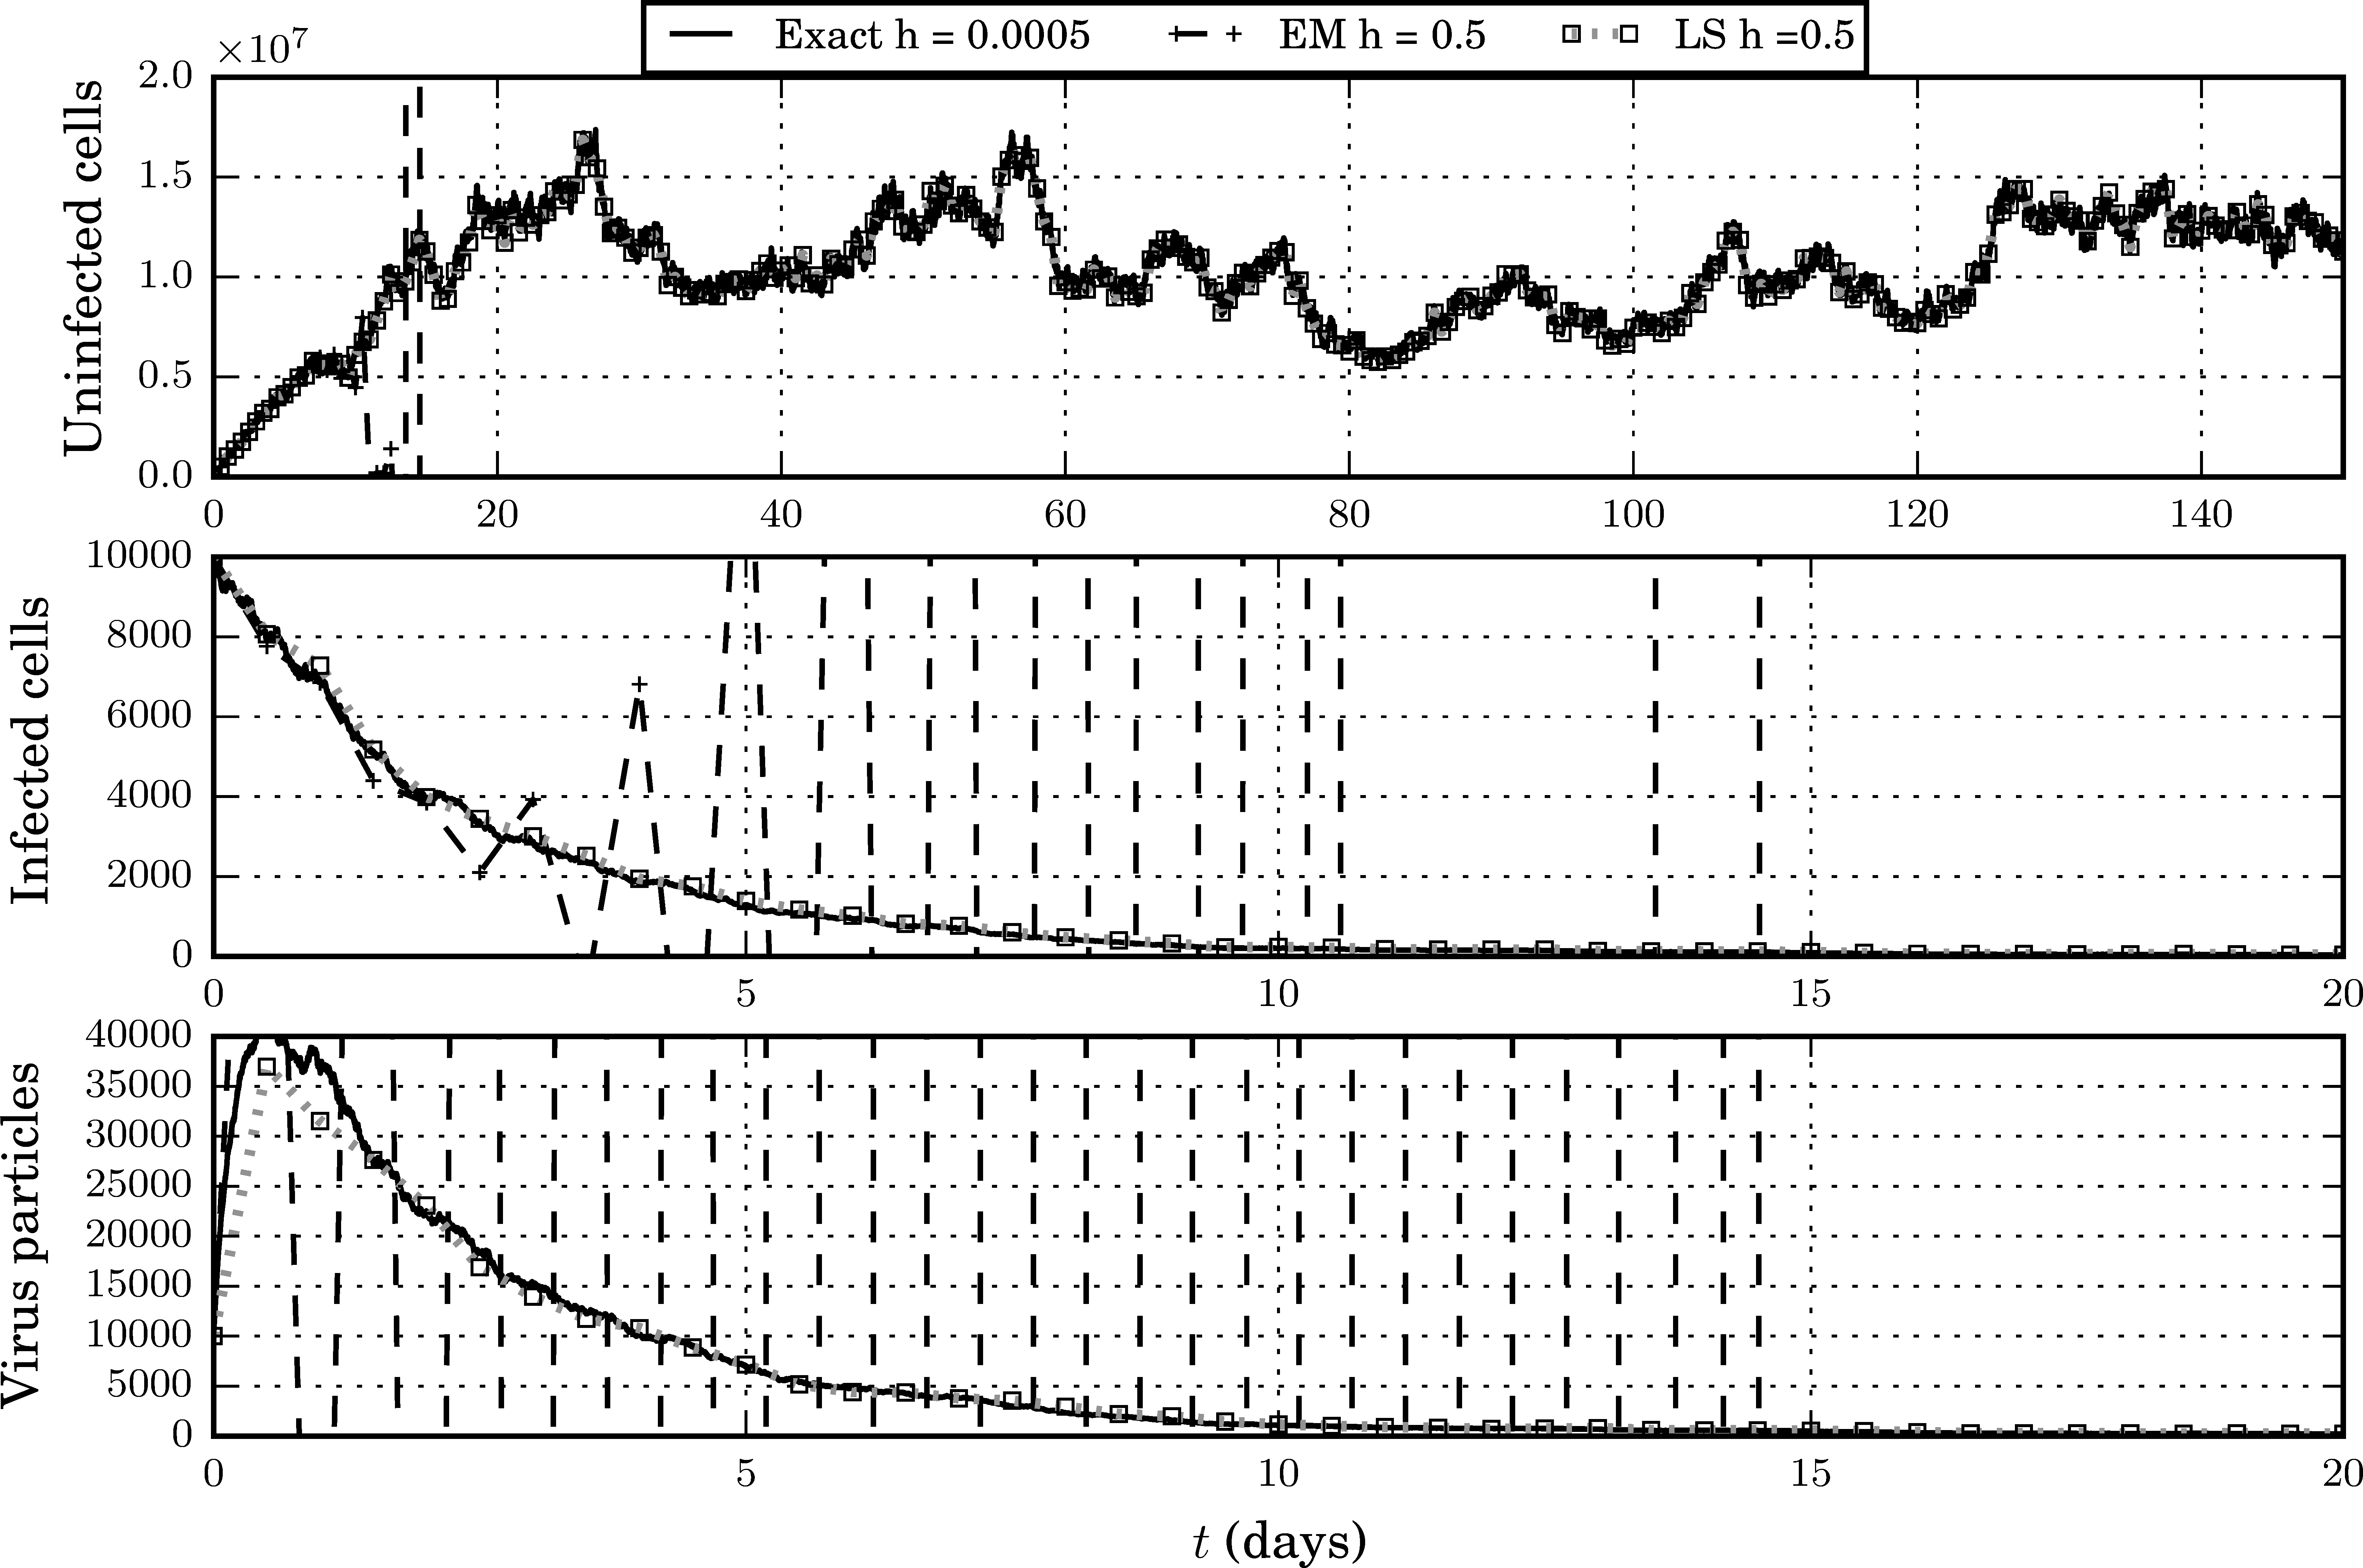
\includegraphics{./papers/paperB/figures/InternalHIVDynamics5e-1.png}
		\caption{
			Likening between EM and SM schemes for SDE \eqref{eqn:StochasticHIVDynamics} with
			$\gamma = \num{0.5}$,
			$\eta = \num{0.5}$,
			$\lambda = \SI{1e6}{\per\cubic\deci\meter\per\day}$,
			$\delta = \SI{0.1}{\per\day}$,
			$\beta = \SI{1e-8}{\cubic\deci\meter\per\day}$,
			$a = \SI{0.5}{\per \day}$,
			$N = \SI{100}{per cell}$,
			$u = \SI{5}{\per\day} $,
			$\sigma_1 = \num{0.1}$,
			$\sigma_2 = \num{0.1} $,
			$X_0 = (\SI{10000}{\per\cubic\deci\meter}, \SI{10000}{\per\cubic\deci\meter}, 
			\SI{10000}{\per\cubic\deci\meter})^T$,
			$h=\num{0.5}$.
			Here the exact solution means a EM simulation
			with the same parameters but with a step-size $h=\num{1e-5}$.
		}
		\label{fig:StochasticHIVDynamicsPaths}
	\end{center}
\end{figure}


	\section{Numerical Methods for Second Order Stochastic Differential Equations}
		In this section we follow the work \cite{Burrage2007} to examine the 
stationary density of the Steklov method and determine how close is from the continuous associated stationary 
density. In due so, we consider the SDE
\begin{align}
	dX_t &= V_t dt \label{eqn:SecondOrderSDE1}\\ 
	dV_t &= -\eta s^2(X_t)V_tdt + f(X_t)dt + \varepsilon s(X_t) dW_t.
	\label{eqn:SecondOrderSDE2}
\end{align}
First we will analyze the case when $s(x)= 1$, and $f(x)$ is linear, we will say
$f(x) = -gx$, $g>0$. In this case this SDE reads
\begin{align}
	dX_t &= V_t dt	\label{eqn:LinearSecondOrderSDE1}\\
	dV_t &= -\eta V_tdt -gX_t dt + \varepsilon dW_t.\label{eqn:LinearSecondOrderSDE2}
\end{align}
The stationary density $\mathbb{P}_\infty$  defined as
\begin{equation*}
	\mathbb{P}_\infty = \lim_{t\to \infty}\mathbb{P}(x,v;t)
\end{equation*}
has the following analytical form, independent of the parameters functions of the SDE and sufficiently 
conditions on the potential $V(x)$
\begin{equation*}
	\mathbb{P}_\infty = N \exp\left(
		-\frac{v^2}{2KT} -\frac{V(X)}{KT}
		\right).
\end{equation*}
So, we will compare three quantities, the mean , the variance and covariance of 
the method with the analytical form. If we consider the linear form the SDE 
\crefrange{eqn:SecondOrderSDE1}{eqn:SecondOrderSDE2}
i.e. \crefrange{eqn:LinearSecondOrderSDE1}{eqn:LinearSecondOrderSDE2} then the corresponding stationary distribution is 
Gaussian and 
takes the form
\begin{equation*}
	\mathbb{P}_{\infty}(x,v) = N \exp
	\left(
	-\frac{gx^2}{2KT}
	-\frac{v^2}{2KT}
	\right).
\end{equation*}
Moreover, the solution of \crefrange{eqn:LinearSecondOrderSDE1}{eqn:LinearSecondOrderSDE2} satisfy
\begin{equation*}
	\lim_{t \to \infty} \left\langle X_t^2\right\rangle = \frac{1}{g}KT, \qquad
	\lim_{t \to \infty} \left\langle V_t^2\right\rangle = KT, \qquad
	\lim_{t \to \infty} \left\langle X_t,V_t\right\rangle = 0.
\end{equation*}
Note that SDE \crefrange{eqn:LinearSecondOrderSDE1}{eqn:LinearSecondOrderSDE2} can be written in matrix notation as
\begin{equation}
	d 
	\begin{bmatrix}
		X_t\\ V_t
	\end{bmatrix}
	=
	Q
	\begin{bmatrix}
			X_t\\ V_t
	\end{bmatrix}
	+ \varepsilon
	\begin{bmatrix}
			0\\ 1
	\end{bmatrix}
	dW_t
\end{equation}
	where
$$
	Q =
\begin{bmatrix}
	0	& 1	\\
	-g	& -\eta	\\
\end{bmatrix}
$$
In this way, we consider numerical updates of the form
\begin{align}\label{eqn:NumericalUpdate}
	&\begin{bmatrix}
		X_{n+1}\\ V_{n+1}
	\end{bmatrix}
	=
	R
	\begin{bmatrix}
		X_{n}\\ V_{n}
	\end{bmatrix}
	+ \varepsilon r \Delta W_n\\
	&R =
	\begin{bmatrix}
		r_{11}	& r_{12}\\
		r_{21}	& r_{22}\\
	\end{bmatrix},
	\qquad 
	r=
	\begin{bmatrix}
		r_1\\
		r_2
	\end{bmatrix}
\end{align}
Since the numerical update \eqref{eqn:NumericalUpdate} is linear in $W_n$ the stationary discrete density 
$\mathbb{P}_{\infty}^{*}(x,v)$ is Gaussian. We take the correlation matrix 
$$
	\Sigma=
	\begin{bmatrix}
		\sigma_x^2,	& \mu\\
		\mu			& \sigma_v^{2}
	\end{bmatrix}
$$
where
\begin{equation}
	\sigma_x^2 = \lim_{n \to \infty} \left\langle X_n^2\right\rangle, \qquad
	\sigma_v^2 = \lim_{n \to \infty} \left\langle V_n^2\right\rangle, \qquad
\mu = \lim_{n \to \infty} \left\langle X_n,V_n\right\rangle .
\end{equation}
Then
\begin{equation}
	\mathbb{P}_{\infty}^* = 
		\frac{1}{2\pi}
		\left|
			\Sigma^{-1}
		\right|^{\frac{1}{2}}
	\exp\left(
		-\frac{1}{2}(x,v)
		\Sigma^{-1}
		\begin{bmatrix}
			x\\v
		\end{bmatrix}
	\right).
\end{equation}
This stationary density has the property of invariance under the linear transformation 
\eqref{eqn:NumericalUpdate}, thus the correlation matrix that results from a numerical method 
satisfies
\begin{equation}
	R \Sigma R^T = \Sigma - \varepsilon^2 r r^T \Delta t.
\end{equation}
Since $\Sigma$ is simetric we can rewrite this equation in a inversion suitable form as
\begin{equation}\label{eqn:MatrixEquation}
	\begin{bmatrix}
		r_{11}^2 - 1	&2r_{11}r_{12}						&r_{12}^2		\\
		r_{11}r_{12}	&r_{11}r_{12}+ r_{12}r_{21} - 1		&r_{11}r_{12}	\\
		r_{21}^2		&2r_{11}r_{12}						&r_{22}^2 -1
	\end{bmatrix}
	\begin{bmatrix}
		\sigma_x^2\\
		\mu\\
		\sigma_v^2
	\end{bmatrix}
	= -\varepsilon^2
	h
	\begin{bmatrix}
		r_1^2\\
		r_1 r_2\\
		r_2^2
	\end{bmatrix}.
\end{equation}
Then solving \cref{eqn:MatrixEquation} we found the stability boundaries of the method  as function
of the parameters $\eta h $, $g h^2$.
For the SSLS method we can write in matrix form the update of the scheme as follows
\begin{equation}
	\begin{bmatrix}
		X_{n+1}\\
		V_{n+1}
	\end{bmatrix}
	=
	\begin{bmatrix}
		1											& h\\
		\frac{g}{\eta}\left(\exp(-h\eta) - 1 \right)	
		& \exp(-\eta h)% + \frac{g}{\eta}\left(\exp(-h\eta) - 1 \right) h 
	\end{bmatrix}
	\begin{bmatrix}
		X_n\\V_n
	\end{bmatrix}
	+
	\varepsilon
	\begin{bmatrix}
		V_n\\
		X_n
	\end{bmatrix}.
\end{equation}
%
Then equation \eqref{eqn:MatrixEquation} reads
\begin{equation}
	\begin{bmatrix} 
		0	&2h		&{h}^{2}\\ 
		\frac{g}{\eta}
			\left( 
				e^{-\eta h}-1 
			\right)
		&
		e^{-\eta h} 
			+\frac{gh}{\eta}
				\left( 
					e^{-\eta h}-1 
				\right) -1
			&
			h  e^{-\eta h}
			\\ 
		\frac{g^2}{\eta^2} 
			\left( 
				e^{-\eta h}-1
			\right)^2
			&
		\frac{2 g}{\eta}
			\left(
				e^{-\eta h} - 1 
			\right)
			e^{-\eta h}
		& 
		e^{-2\eta h} -1
	\end{bmatrix}
	\begin{bmatrix}
		\sigma_x^2\\
		\mu\\
		\sigma_v^2
	\end{bmatrix}
	=
	\begin{bmatrix}
		0\\
		0\\
		\epsilon^2 h
	\end{bmatrix}.
\end{equation}
Hence, solving we get
\begin{equation}
	\begin{bmatrix}
		\sigma_x^2\\
		\mu\\
		\sigma_v^2
	\end{bmatrix}
	=
	\frac{2 K T  \eta^3}
	{
		\left( \eta-g h \right)
		\left(e^{-\eta h}-1 \right) 
		\left( 
			2 e^{-\eta h}\eta
			-gh e^{-\eta h}
			+gh
			+2 \eta
		\right)
	}
	\begin {bmatrix}
		\frac{
			\left(
			 e^{-\eta h}\eta
				-gh e^{-\eta h}
				+gh
				+\eta 
			\right)
		}{
			g ( e^{-\eta h}-1)
		}\\ 
		h^2\\ 
		-2h
	\end {bmatrix}.
\end{equation}
Comparing with the correlation matrix for the Euler-Maruyama method 
\begin{equation}
	\Sigma_E = 
	\frac{KT}{1-\frac{g}{\eta}h}
	\left(
		2-\eta h +\frac{1}{2} g h^2
	\right)^{-1}
	\begin{bmatrix}
		g^{-1}(2-\eta h +g h^2) & -h\\
		-h &	2
	\end{bmatrix}
\end{equation}
we can see that the correlation between $X_t$,$ V_t$ is ${o}(h)$ while that for the SSLS is 
$o(h^2)$. In \Cref{fig:MeanSquareEta} we show the difference between the exact and the theoretically 
moments of the Euler and SSLS methods.
\begin{figure}[htb]
	\centering
	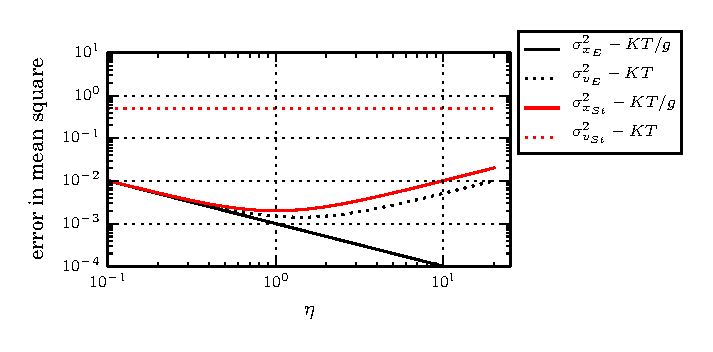
\includegraphics{./papers/paperB/figures/ErrorVariances.eps}
	% ErrorVariances.eps: 0x0 pixel, 300dpi, 0.00x0.00 cm, bb=0 0 256 158
	\caption{Difference between the calculated moments and analytical form versus $\eta$ parameter. Here
	$g=1$, $K = 1$,$T = 1$, and $h =\num{0.1}$.}
	\label{fig:MeanSquareEta}
\end{figure}

	\section{Linear Oscillator}
			This model was studied in \cite{Melbo2004}.
		Melbø Aslaug, H. Strømmen, Higham Desmond. 
		Numerical simulation of a linear stochastic oscillator with additive noise
			\begin{align}
				dx(t) &= y(t)dt\\
				dy(t) &= -x(t)+h dW(t) \qquad h>0.
			\end{align}
		The Steklov Scheme is under construction.
	%\section{Path-wise stability for Additive Noise}
		%We will start our analysis using a unidimensional SDE
\begin{equation}\label{eqn:1-dSDE}
	dX_t = f(X_t)dt +\sigma dW_t, \qquad \sigma>0,
\end{equation}
where f can be written as
\begin{equation}
	f(x) = a_1(x)x + a_2.
\end{equation}
Also, we will assume sufficiently conditions about $f$ to existence and uniqueness of solutions. Moreover, we will
assume that $a_1$  takes at most a countable set of points where vanishes. Under this assumptions we write a
Quasilinear Steklov Scheme (QSS) as
\begin{equation}\label{eqn:QSS}
	X_{k+1}=
		\left(
			X_k + \frac{a_2}{a_1(X_k)}
		\right)
		\exp
		\left(
			 h a_1(X_k)
		\right)
		-\frac{a_2}{a_1(X_k)}
		+\sigma \Delta W_k.
\end{equation}

In order to study asymptotic pathwise stability we will assume that $f$ satisfies a one sided Lipschitz condition
\begin{equation}
	\left <
		x-y, f(x)-f(y)
	\right> 
	\leq
	-L|x-y|^2 ,\qquad L>0, \qquad x,y \in \mathbb{R}.
\end{equation}
Our goal is to determine conditions to assure numerical pathwise stability when the QSS scheme is applied. To deal
with this, we have to verify bought, that two numerical solutions of the scheme \eqref{eqn:QSS} 
$X_n,Y_n$ are absorbed in the limit  when
$t_n \to \infty$, i.e, 
$$
|
	X_{n}^{(1)}
	- X_{n}^{(2)}
|\to 0, \qquad t_n \to \infty
$$
and show the existence of a random attractor.
So, under the above assumptions we have
\begin{align*}
	|X_{n+1}- Y_{n+1}|^2
	& =
	\left<
		X_{n+1}-Y_{n+1},
		X_n \exp \left(h a_1(X_n)\right)
		-Y_n \exp\left(h a_1(Y_n)\right) 
	\right>	\\
	&+
	\left<
		X_{n+1}-Y_{n+1},
		\frac{a_2 \exp(h a_1(X_n))}{a_1(X_n)} 
		-
		\frac{a_2 \exp(h a_1(Y_n))}{a_1(Y_n)}
	\right>	\\
	&-
	\left<
		X_{n+1}-Y_{n+1},
		a_2
		\left(
			\frac{1}{a_1(X_n)}
			-\frac{1}{a_1(Y_n)}
		\right) 
	\right>	.\\
\end{align*}
By Cauchy-Schwartz inequality follows
\begin{align*}
	\left|X_{n+1}- Y_{n+1}\right|
		&\leq	
		\left|
			X_n \exp \left(h a_1(X_n)\right)
			-Y_n \exp\left(h a_1(Y_n)\right) 
		\right|	\\
		&+
		|a_2|
		\left|
			\frac{\exp(h a_1(X_n))}{a_1(X_n)} 
			-
			\frac{\exp(h a_1(Y_n))}{a_1(Y_n)}
		\right|	\\
		&-
		|a_2|
		\left|
			\frac{1}{a_1(X_n)}
			-\frac{1}{a_1(Y_n)}
		\right|
\end{align*}

	\clearpage
	\section*{\refname}
	\bibliographystyle{model2-names}
	\bibliography{library,Books}
\end{document}